%% NOTE: The LaTeX format of this template is the authoritative version, but if you 
%% wish you may convert it to, e.g., Word or Google Docs format for editing. Recent 
%% versions of Word and LibreOffice can natively edit PDF files, as can Google Docs
%% (with minor formatting issues you will need to correct). Alternatively, you can use 
%% pandoc (and other free online conversion tools such as those listed here: 
%% https://softwarerecs.stackexchange.com/questions/1361/)

% Global template configuration (see custard.cls for details)
% Two-sided means the left and right margins are different sizes and they alternate 
% every page. If your document is printed to be book or spiral bound this allows for a 
% thick spine that does not eat into the space for your page content. 
% You can also add "draft" as an option if needed, which clearly marks the document 
% as a draft, hides the declaration, dedication, acknowledgements and appendix, 
% and forces one-sided mode to save space.
\documentclass[11pt, a4paper, oneside, openright]{custard}



% All imports, packages and configuration go in here. Your document should be 
% about content, so we abstract away the styling rules and tools we are using. 
% !TEX root = thesis.tex
%% Here you can specify new packages, commands and environments that you intend
%% to use. Using custom commands (for example, those for e.g., i.e., etc. below)
%% can make your document easier to write, read and more consistent.
\usepackage{float} % Adds the [H] option for forced figure placement
\usepackage[norefs,nocites]{refcheck} % Check and warn about unused labels
\usepackage[export]{adjustbox} % Used to add a frame around figures

% We are writing in British English
\usepackage[british]{babel}

% How many levels of sections/subsections etc to display in the Table of Contents
\setcounter{tocdepth}{1}

% Space out lines slightly - 1.5 spacing is overly severe, so we go for a 
% more visually pleasing 1.31
\linespread{1.31}

% Paragraph spacing
\setlength{\parskip}{0.5em}

% Common shortcuts for consistency - this allows you to write, for example, 
% \eg in LaTeX instead of typing e.g., so that every single instance will be 
% formatted identically. If you later want to change one of these definitions, 
% all usages throughout the document will be updated.
\newcommand{\eg}{e.g.,\xspace}
\newcommand{\ie}{i.e.,\xspace}
\newcommand{\etc}{etc.\@\xspace}
\newcommand{\cf}{cf.\xspace}
\newcommand{\vs}{vs.\xspace}
\newcommand{\etal}{et al.\xspace}
\newcommand{\sd}{s.d.\xspace}
\newcommand{\elide}{[\,\ldots]\xspace}
\newcommand{\edots}{\,\ldots}

% Figure caption formatting
\usepackage[font=small,skip=1em]{caption}
\usepackage[labelformat=simple]{subfig}
\renewcommand{\thesubfigure}{\alph{subfigure})}

% Allow multiple columns
\usepackage{multicol}
\usepackage{enumitem}

% Put footnotes at bottom of page always
\usepackage[bottom]{footmisc}

% Code listing formatting
\usepackage[final]{listings} % "final" option means show listings even in draft mode
\usepackage{lstautogobble}
\usepackage{sourcecodepro}
\pdfmapfile{=SourceCodePro.map}
\lstset{
	xleftmargin=0.5cm,frame=tlbr,framesep=4pt,framerule=0.5pt,
	language=,
	upquote=true,
	columns=fixed,
	tabsize=2,
	extendedchars=true,
	breaklines=true,
	numbers=left,
	numbersep=10pt,
	basicstyle=\ttfamily\scriptsize,
	numberstyle=\tiny,
	stringstyle=\ttfamily,
	captionpos=b,
	showstringspaces=false,
	autogobble=true
}



% Use IEEEtran citation style
\bibliographystyle{IEEEtran} 


\begin{document}
% The custom data for Swansea University and your degree.
% Your name and (for all except Doctoral theses), your student number
	\title{Initial Document: A Multifunctional Fitness Application \& Vertical Jump Height Calculator}
	\author{Rowan Aldean}
	\studentnumber{973765}
	\awardinginst{Swansea University}
	
% Comment / uncomment your degree type as needed.
	\degree{BSc (Hons) Software Engineering w/ Year in Industry} 
	% \degree{Master of Science}
	%\degree{Doctor of Philosophy}
	
% Institution details and logo
	\department{Department of Computer Science}
	\university{Swansea University}
	\unilogo{swansea-logo.pdf}
	
% Hard code the date or allow the LaTeX compiler to fill it in 
% whenever you recompile the document.
	\date{20th October 2021}
	%\date{\today}
	
% Build the title and declaration pages, and pad the document so the text starts 
% on a right-hand book page. Page numbering is in roman numerals until the first 
% page of an actual chapter, which resets numbers starting from 1 at that point. 
	\frontmatter
	\maketitle
	\declaration
	\cleardoublepage
	
% Most significant books and theses have a brief foreword or dedication. 
% Shorter documents normally do not - remove / comment out if necessary.
	% \ifdraftdoc\else
	% \begin{vplace}[0.7]
	% 	\begin{large}
	% 		\begin{center}
	% 			\textit{I would like to dedicate this work to\edots}
	% 		\end{center}
	% 	\end{large}
	% \end{vplace}
	% \fi

% The abstract comes before the contents page. Note how each sentence is 
% written on a new line - this is an optional convention that can make it easier 
% to compare versions of your document using automated tools (e.g., diff).
% 	\begin{abstract}
% 		\vspace{-2em}
% 		\setcounter{page}{1}
% In your abstract you should aim to summarise the core contributions of your work in the context of the problem domain.
% Start by outlining the domain and the problems posed within it.
% Discuss how the methods you focus on approach the relevant problems.
% You should end your abstract by concretely stating the tangible outputs and deliverables you have created in order to complete your work on this document, and whether those outputs represent and improvement or alternative approach to existing methods.

% Your abstract should be a couple or so paragraphs long, and roughly approximate the order and flow you then use for structuring the main document.
% If a viewer has read your abstract then they should already understand at a high level what it is you have created and delivered, and whether it is better than or comparable to existing methods.
% If your project is driven by a research hypothesis then the reader should know what that is at a high level from this section.
% Reading on, little should surprise the viewer.

% For paper submission of your thesis you should physically sign your name and add the date for each of the above declaration statements (black ink preferred).
% For digital submissions it is normally enough to simply type your name (see custard.cls), though you should sign and date them digitally using a touch or stylus input if at all possible.
% 	\end{abstract}
	
% % A long form dedication (optional).
% 	\ifdraftdoc\else
% 	\begin{Acknowledgements}
% This is an opportunity to acknowledge and thank those who have supported you throughout your studies.
% Friends and colleagues who you have studied alongside, your families, and your mentors within the department are the usual suspects. 
% 	\end{Acknowledgements}
% 	\fi
	
% Build the table of contents page.
	\tableofcontents*
	 
% Optionally you can make a bank of known acronyms in acronyms.tex that you can call on throughout your document.
	%\input{acronyms} 
	
% For long documents like a Doctoral thesis you often include a list of tables and 
% figures that are used throughout your document. The command below uses a
% shortened version of each table and figure caption (specified by you - see examples 
% throughout) and enumerates all of them with their table or figure number. This 
% process is automatic - just uncomment the lines below to use it.
	%\newpage
	%\listoftables
	%\mtcaddchapter 
	%\newpage
	%\listoffigures
	%\mtcaddchapter

% If you use todo notes, you want to make sure you fix them all before final submission
	\ifnum\totvalue{todocounter}>0
		\listoftodos
	\fi

% Reset numeric page numbering from page 1
	\mainmatter

% Insert the source file for each of your chapters
	% !TEX root = ../thesis.tex
\chapter{Introduction}
\raggedright
\label{chap:intro}
This document will outline the plan for development of a functional codebase for a fitness application.
This process, herein referred to as ``the project'' is different to the application(s) produced as a result.
The main difference is that the project is not concerned with the deployment, maintenance and future updates
of the fitness application and no additional academic benefit is gained from creating the
infrastructure or platform-specific functionality. This is to say that the creation
of \textbf{both} a mobile and a web application is not needed for the project but makes up
a core offering of the product for end users following deployment.
\par
\noindent
A \textbf{mobile} application will be produced during the project, which will have 2 main use cases:
\begin{enumerate}
	\item A user will be able to pay (via monthly installments or upfront) for a
	      fitness plan; where they can monitor, make notes and track their
	      progress and routine via a calendar.
	\item A user can create their own fitness plan by producing their own routine using
	      available exercises on the app - the additional functions such as the calendar remain
	      the same.
\end{enumerate}
\pagebreak
\section{Motivations}
\label{sec:intro_motivation}
\hyphenpenalty=100000
The motivation for the project began following an initial consultation with a Californian
NBA-level basketball athletic trainer who was looking for a bespoke application
to reduce his business expenses. Initially, 4 days of planning and a 40-minute discussion
took place before the business decided that the costs associated with building this platform
are not a priority for the time being.
\par
In the process of considering the development of said fitness platform, I spoke to developers
working with smaller high-level sports trainers regarding the technology used and their clients
future plans. At this time fitness influencers Krissy Cela and Jack Bullimore had proven the concept
a year earlier with the rollout of ``\href{https://toneandsculpt.app/}{Tone and Sculpt}'' -
grossing over GBP 1 million in the 8 months following its January 2019 release \cite{tonensculpt}.
My initial desire to pursue a project in this space grew more after hearing the story and approach taken by
``Tone and Sculpt'' on the Diary of a CEO podcast \cite{krissy-podcast}.
\par
In the world of athletic sports there is currently no viable, consistent and widely used means
of measuring vertical leap besides
\href{https://www.topendsports.com/testing/products/vertical-jump/vertec.htm}{the Vertec}.
Prices on these devices can be as high as £500 and cheaper alternatives commonly found
at a youth/amateur level - that involve markings on walls - don't allow for an approach
jump (without the risk of hitting the wall). This is being mentioned because a large motivation for the jump calculator
functionality is to allow an easy and accessible means of measuring a users vertical leap
progress. Naturally, the use of a smartphone for measurement is not completely accurate but
will provide sufficient consistency (given the user's setup) and this can be used to monitor
improvement.
\par
From a trainers' perspective,  using PDFs to release fitness plans is cumbersome
and involves finding a suitable workflow and rollout. Further to the fact that they're
easily copied and distributed. Existing white-label\footnote{A white-label product is a product or service produced by one company that other companies rebrand to make it appear as if they had made it.}
 mobile app solutions to these issues
don't offer much customization beyond simple re-branding; many don't support video.
Following discussion with fitness trainers in various countries (including the USA, UAE and UK)
I concluded that this is something that needs to be addressed. Many robo-fitness apps
exist for end users, but few include real trainers and even less give
freedom to the administrator.
\par
In summary, the motivation for the project is to give a customizable fitness planning
solution to those interested in monitoring their training. This solution should be
usable by administrators (trainers/teams), average ``gym go-ers'' and
highly trained athletes alike. The global fitness app market size
was valued at USD 4.4 billion in 2020 and is expected to expand at a
compound annual growth rate (CAGR) of 21.6\% from 2021 to 2028 \cite{fitness-app-market-size}.
We can see that the total addressable market is huge and set to grow quickly,
if this is any indicator of the volume of potential users looking for a fitness solution then the proposed
project should prove tremendously useful at solving the aforementioned problems.
\pagebreak

\section{Overview \& Aims}
\label{sec:intro_overview}
The projects aims include the following - some of these aims will be broken down into
succinct functional and non-functional requirements in \cref{sec:requirements}:
\begin{itemize}
	\item The ability for a user to plan their workouts on a calendar.
	\item The ability for a user to track the progress of a workout.
	\item The ability for a user to measure their vertical leap using their phone.
	\item Allow users to keep track of their progress in relevant areas
	      such as weight, strength measurements etc. more efficiently than traditional methods.
	\item Allow trainers to comfortably deliver fitness plans to
	      clients without a steep technical learning curve.
\end{itemize}
The core overview of the project is that we're looking to develop a mobile application that
allows a user to register an account before having the ability to follow/create a fitness plan
and provide relevant tools for consistency and the successful reach of a users goals
(irrespective of their background). The project aims to focus on the 
end user\footnote{The user training using the app} however considerations will be made for 
the complete implementation of an administrator role (time permitting).
\par
The project is concerned with the ability to solve both parties problems through the development
of the application, but the primary focus is on the development of the core functionality
and the vertical jump calculator. From a business perspective we can consider the jump calculator
the unique selling point of \textit{the product} and
a complex component of \textit{the project}.

	% !TEX root = ../thesis.tex
\chapter{Project Research}
\label{chap:research}
We've previously seen that ``Tone \& Sculpt'' is an existing similar application
on the market. Below we'll consider other background research on existing
systems and their functionality.

The bulk of fitness mobile applications fall into 2 categories:
\begin{enumerate}
	\item Applications which allow fitness enthusiasts to monitor their training
	      and nutrition - the market leaders in this space
	      (by monthly active users) are ``Fitbit''
	      and ``My Fitness Pal'' (as of March 2018) \cite{statista-monthly-users}.
	\item Applications which allow trainers to facilitate the delivery of programmes
	      either by partnering with the development company or white-labelling software.
	      These are apps focused on trainers more than end users - the most notable player
	      in this emerging market would be ``TrueCoach''\href{https://truecoach.co/} , who
	      raised USD 2.6 million in seed round funding before being
	      acquired by TSG (Transaction Services Group) in April 2020 \cite{truecoach-funding}.
	      Estimated revenue over USD 1.2 million (from 20k users) for 2021 \cite{truecoach-revenue}.
\end{enumerate}

We can see the main difference in these groups are that
the focus of the former is B2C (business-to-consumer) services
whereas the latter focus on B2B (business-to-business; often acting as SaaS companies).
This is an important distinction as \textit{the project} is looking to combine elements
of both and so the following research will reflect this.
\par
We'll also look at vertical jump calculators and the mathematics involved in developing
something of that nature.
\pagebreak

\section{Existing fitness application systems}
We'll look at 4 systems, 2 from each of the aforementioned application groups. Here it is
worth mentioning that some apps are on the borderline such as
``Centr by Chris Hemsworth''\href{https://centr.com/}. The app follows a B2C approach
but is marketed and part-owned by Chris Hemsworth, with his trainers being the facilitators of programmes
and nutrition plans. A similar approach to the aforementioned
\hyperref[sec:intro_motivation]{``female-focused Tone \& Sculpt''}.
Because cases like these are not relevant to the application being built
for the project, we will not look in any depth at these.
\par
For each of these systems we'll be looking at:
\begin{itemize}
	\item A typical user story for the given application.
	\item A high-level breakdown of the system(s) functionality.
	\item A look at the technology in use (where possible).
\end{itemize}
We'll then compare the applications (in pairs) to see any unique features
and to understand which functions are seemingly core to a positive user experience
in the fitness application space.

\subsection{MyFitnessPal}
\begin{figure}[H]
    \centering
    \begin{minipage}{0.5\textwidth}
        \centering
        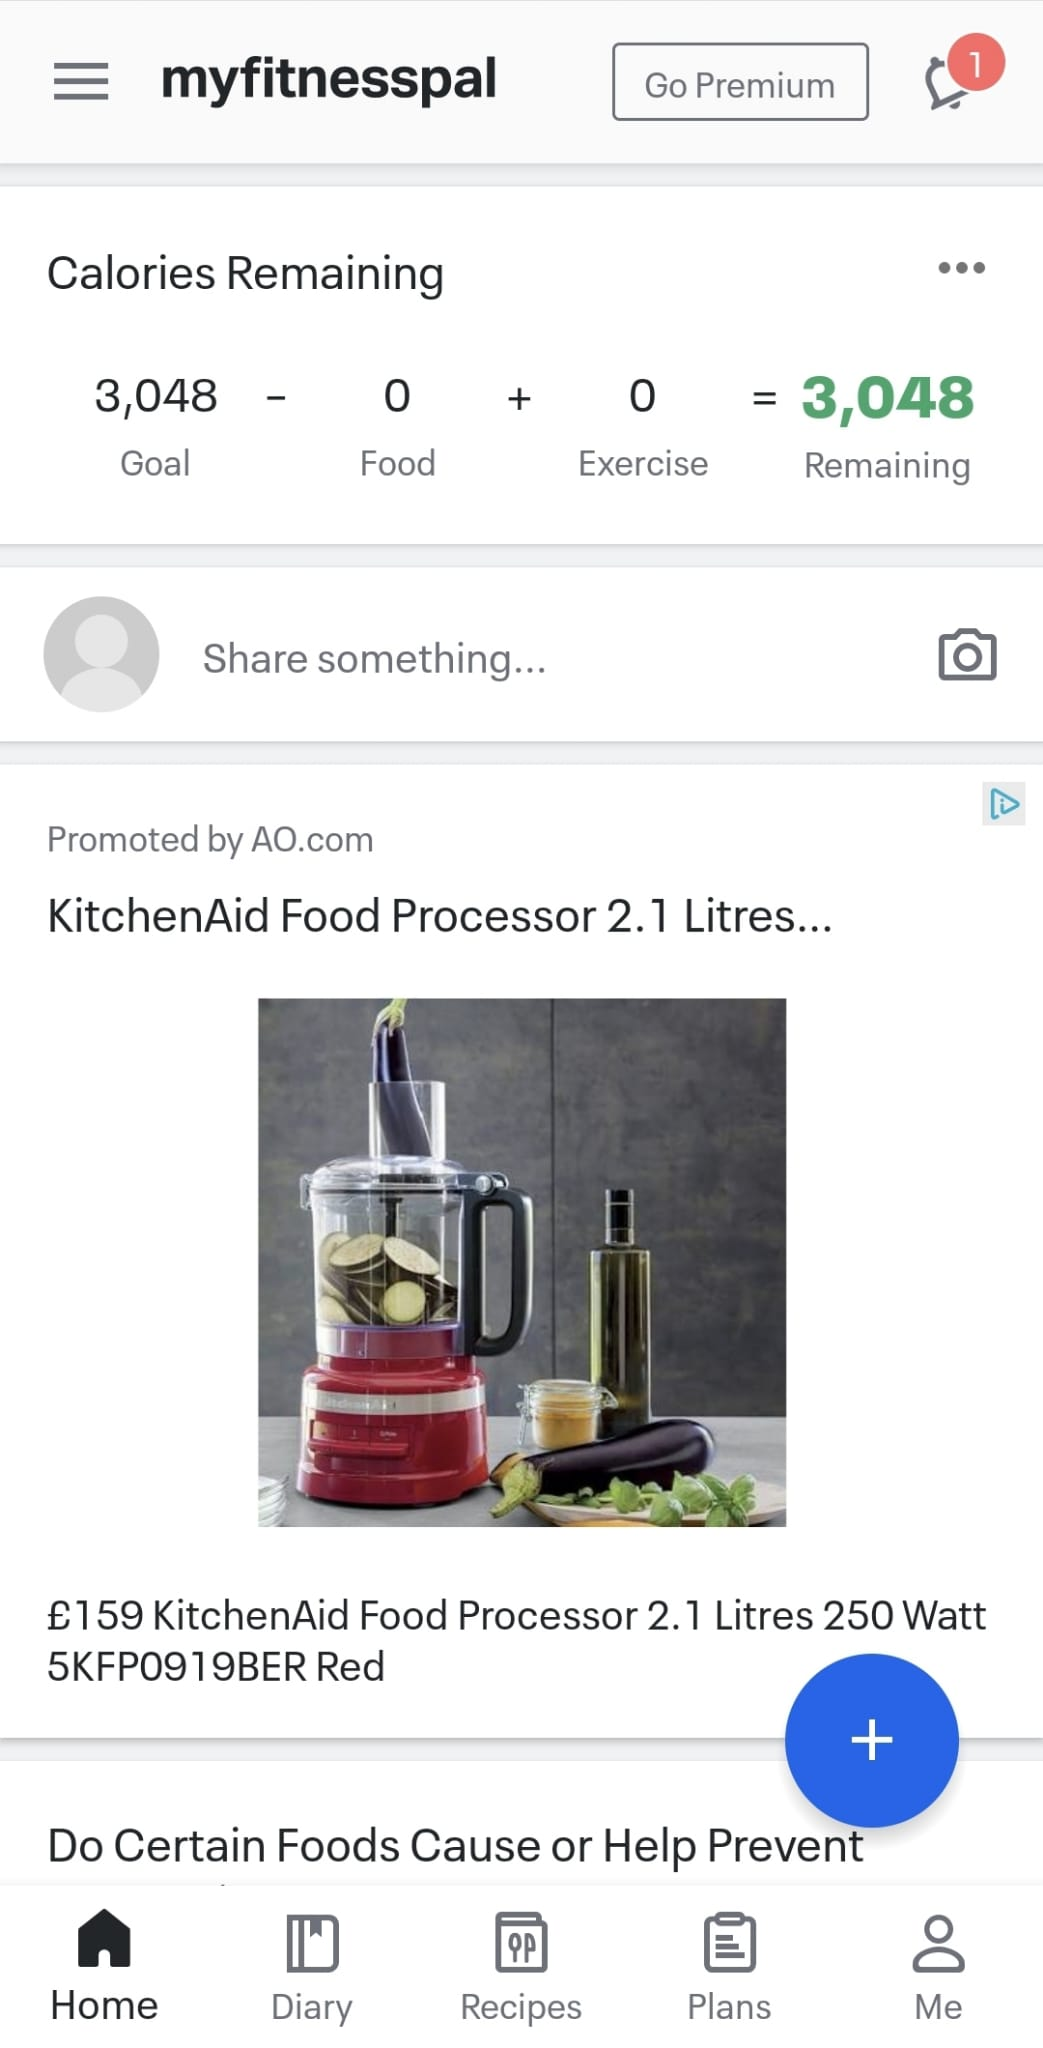
\includegraphics[width=0.5\textwidth]{myfitnesspal/homepage.jpeg}
        \caption{Homepage feed}
        \label{fig:mfp-home}
    \end{minipage}%
    \begin{minipage}{0.5\textwidth}
        \centering
        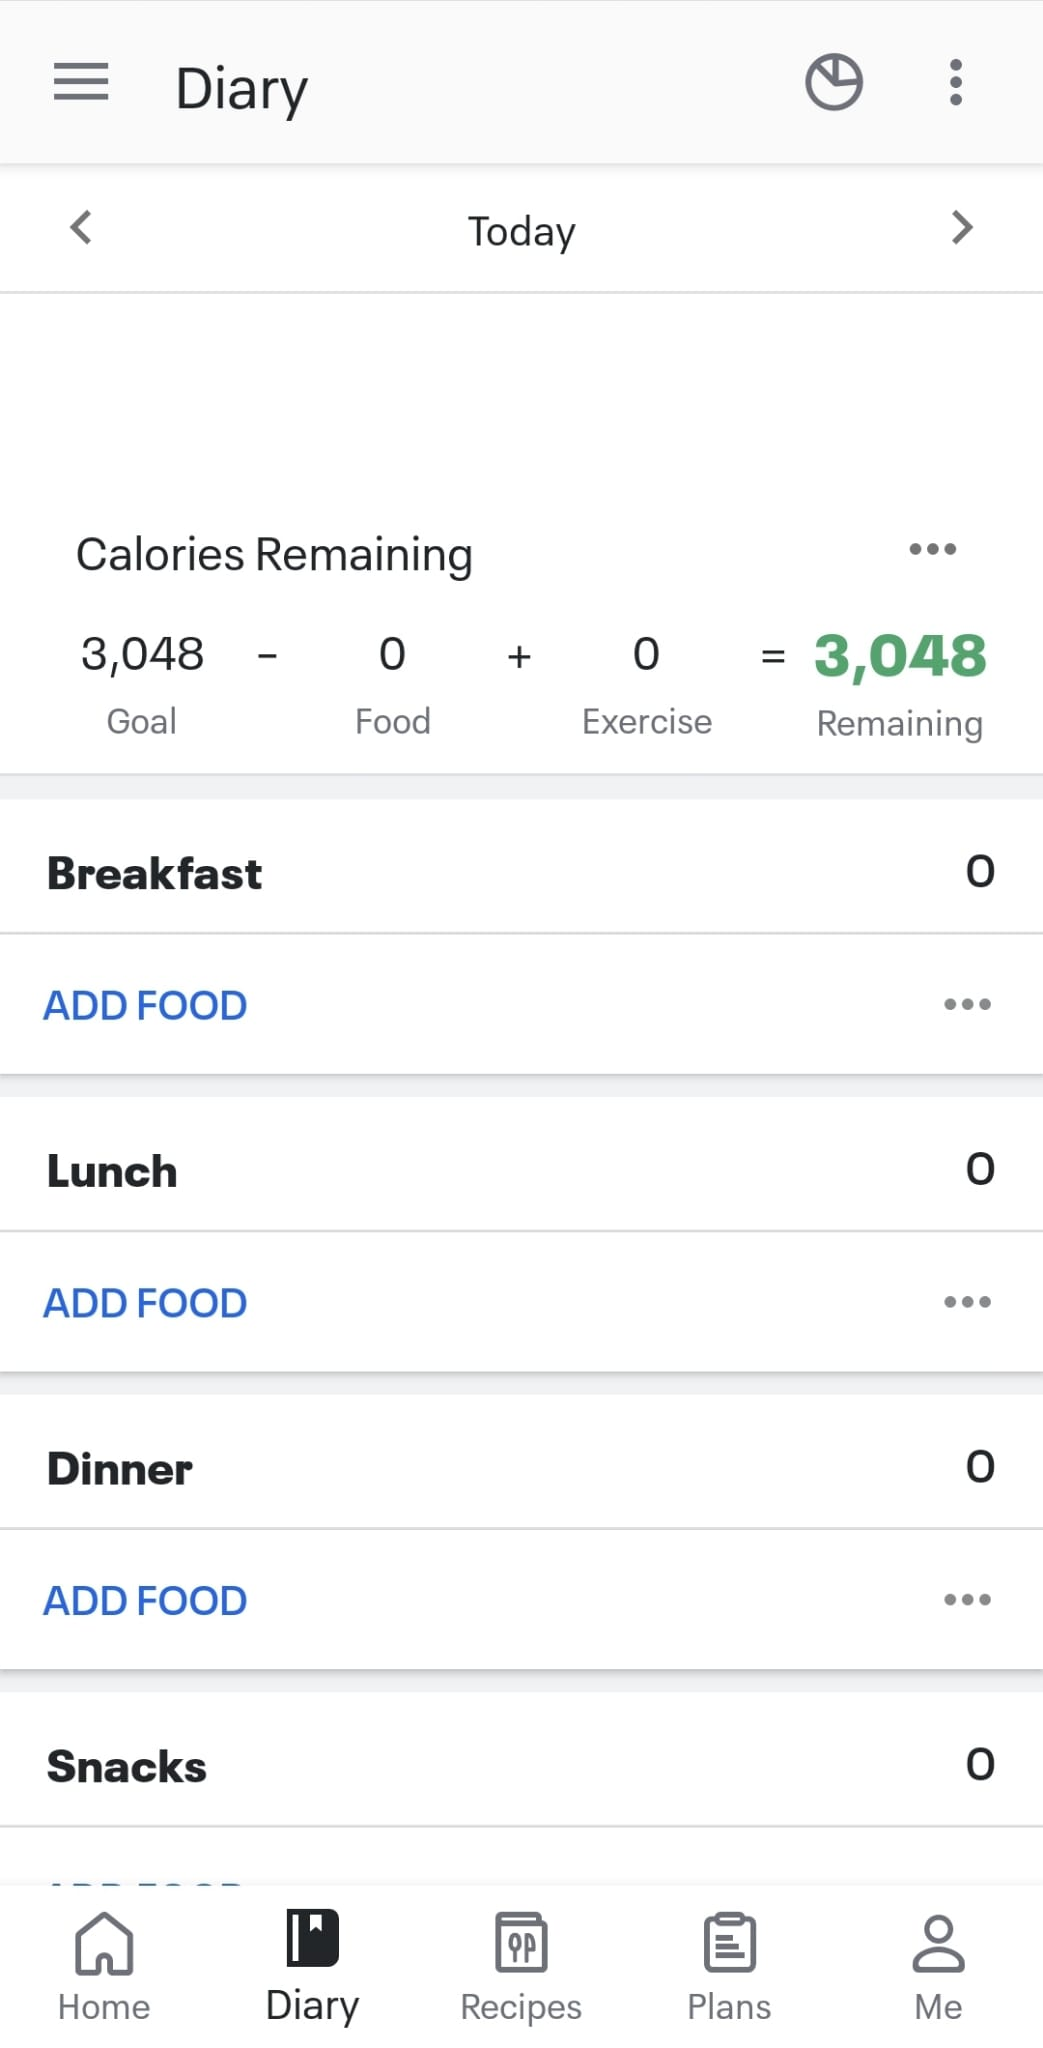
\includegraphics[width=0.5\textwidth]{myfitnesspal/calorie-counter.jpeg}
        \caption{Food diary \& calorie counter}
        \label{fig:mfp-diary}
    \end{minipage}%
\end{figure}
\textbf{User Story}
\label{research-breakdown:mfp-usr-story}
\par
``As a fitness enthusiast, I sign up to the app via email. I wake up
every day and log my breakfast by scanning barcodes for my food.
This is accounted for in my daily food tracking (\cref{fig:mfp-diary}).
After breakfast I create a new workout based on advice from my community or homepage,
I search for the exercises involved and log my workout later on in the day (\cref{fig:mfp-screens}).''
\begin{figure}[H]
    \begin{minipage}{0.5\textwidth}
        \centering
        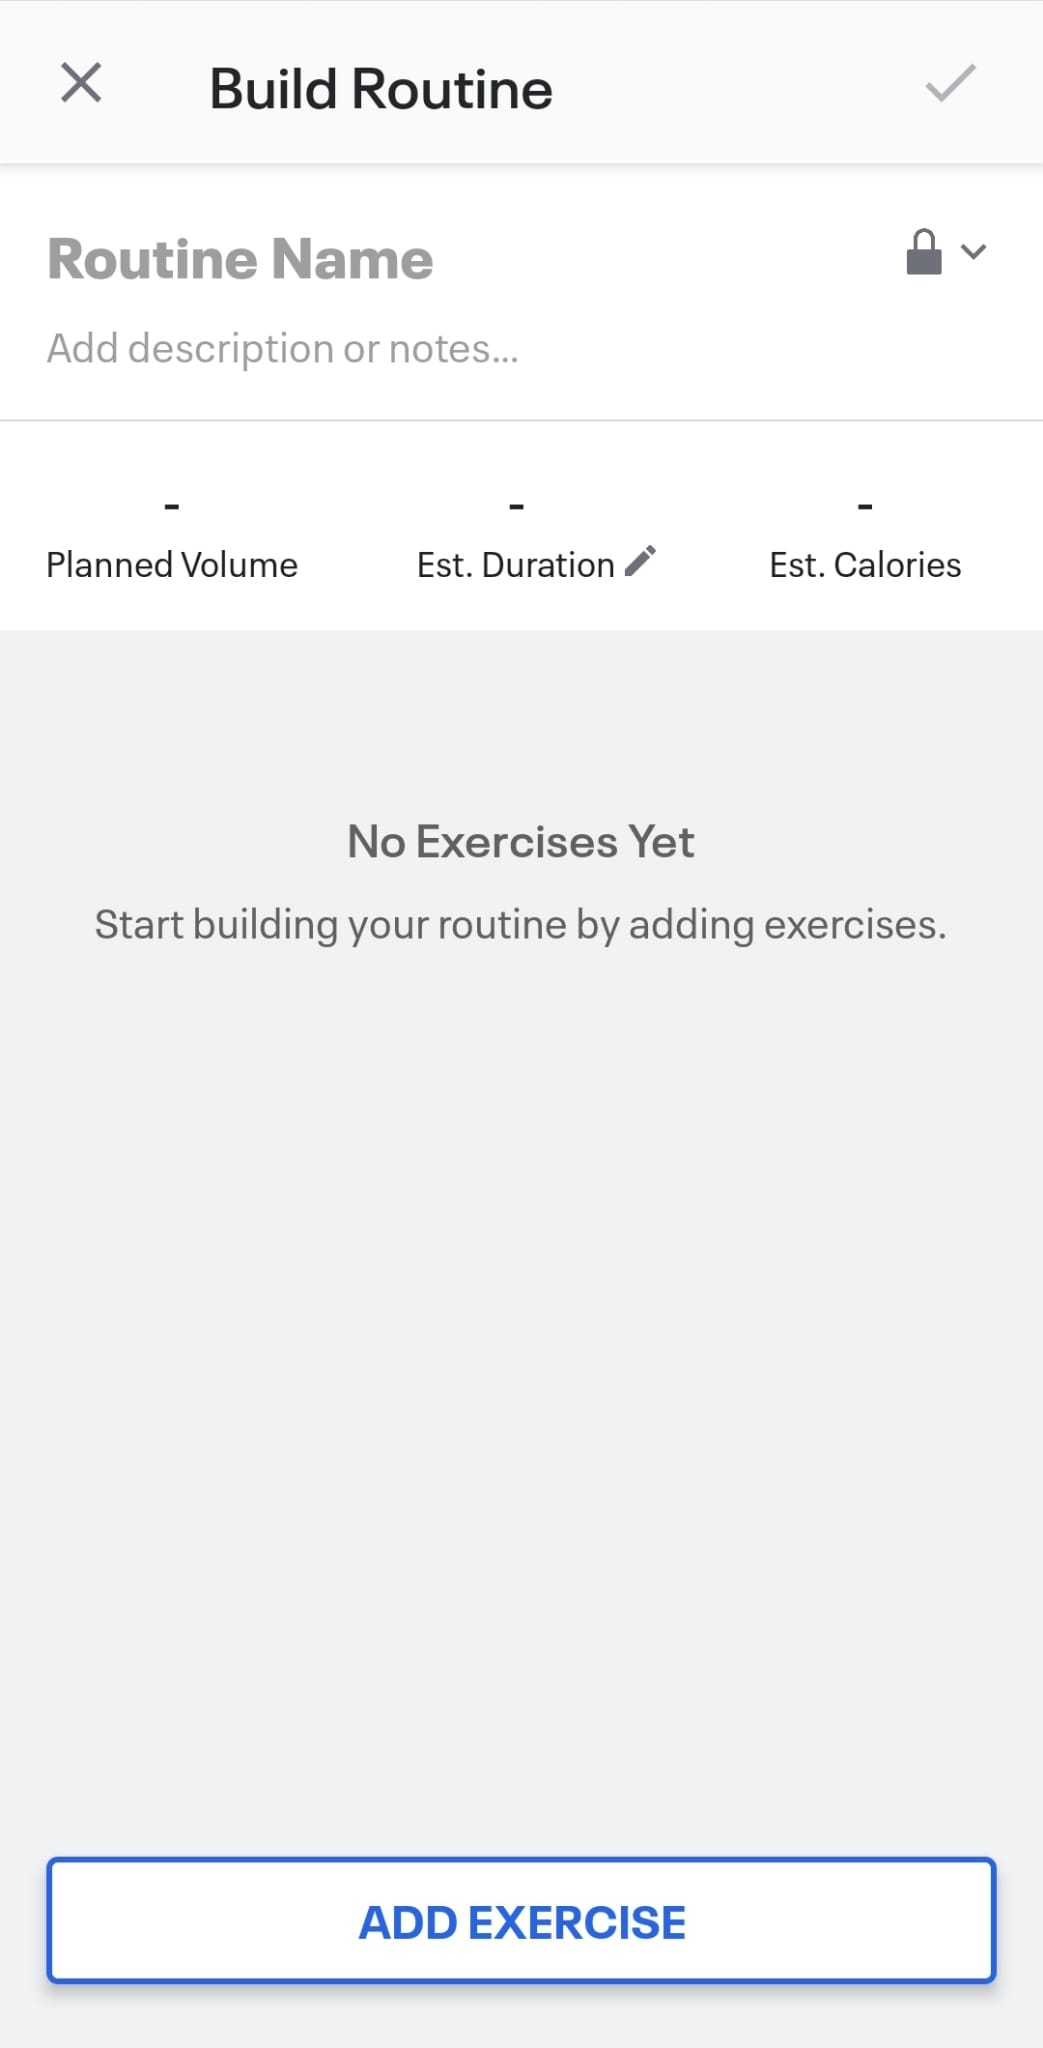
\includegraphics[width=0.5\textwidth]{myfitnesspal/exercise-routines.jpeg}
        \label{fig:mfp-workouts}
    \end{minipage}%
    \begin{minipage}{0.5\textwidth}
        \centering
        \includegraphics[width=0.5\textwidth]{myfitnesspal/exercise-choice.jpeg}
        \label{fig:mfp-exercise-picker}
    \end{minipage}
    \captionof{figure}{The custom workout routines in MFP}
    \label{fig:mfp-screens}
\end{figure}
\textbf{Features/Functionality}
\label{research-breakdown:mfp-features}
\par
MyFitnessPal includes all of the following features:
\begin{multicols}{2}
	\setlist{nolistsep}
	\begin{itemize}[noitemsep]
		\item Estimate calories burned given a set of exercises/a routine.
		\item Track food intake via barcode scan or recipe input.
		\item Track water.
		\item Workout plans provided by MFP.
		\item Track weight.
		      \columnbreak
		\item Create custom workout plans from existing exercises.
		      \setlist{nolistsep}
		      \begin{itemize}[noitemsep]
			      \item Exercises don't include video/images and no ability to add custom exercises.
			      \item These can be shared publically to dashboard.
		      \end{itemize}
		\item Count steps (using compatible devices).
		\item Add friends and send/receive messages.
		\item Community tab (requires separate signup).
		\item Export progress as CSV.
		\item Meal and weight tracking reminders (via push notifications).
		\item Set workout/week, minutes/workout and ``calories burned'' goals.
		\item Discover recipes/meal plans via community and MFP suggestions.
	\end{itemize}
\end{multicols}
\textbf{Technology Stack}
\label{research-breakdown:mfp-stack}
\par
MyFitnessPal uses the following technologies according to Stackshare \cite{mfp-stack}:
\begin{itemize}
	\item React (a JavaScript framework for creating cross-platform applications)
	\item Cloudflare (for web infrastructure)
	\item NginX (for server side use)
	\item Vanilla JavaScript and CSS + libraries (jQuery, Bootstrap)
\end{itemize}
Various other technologies are being used on the server-side but for \textit{the project}
we are primarily concerned with the technology used for the application
as opposed to the backend infrastructure.


\subsection{Fitbit}
Fitbit is the app that accompanies many of the Fitbit brands'
hardware products, their first movers advantage was likely
a large contributor towards their large market share (in 2018)\footnote{Q3 2020 wearables market share = 2.6\%\cite{fitbit-market-share}}
in the application space.
The functionality of their hardware products (which had been the standard for
fitness tracking wearables)
is enhanced through use of the app. The research will consider the application alone and disregard
any wearable-specific functionality.
\pagebreak
\begin{figure}[H]
    \begin{minipage}{0.5\textwidth}
        \centering
        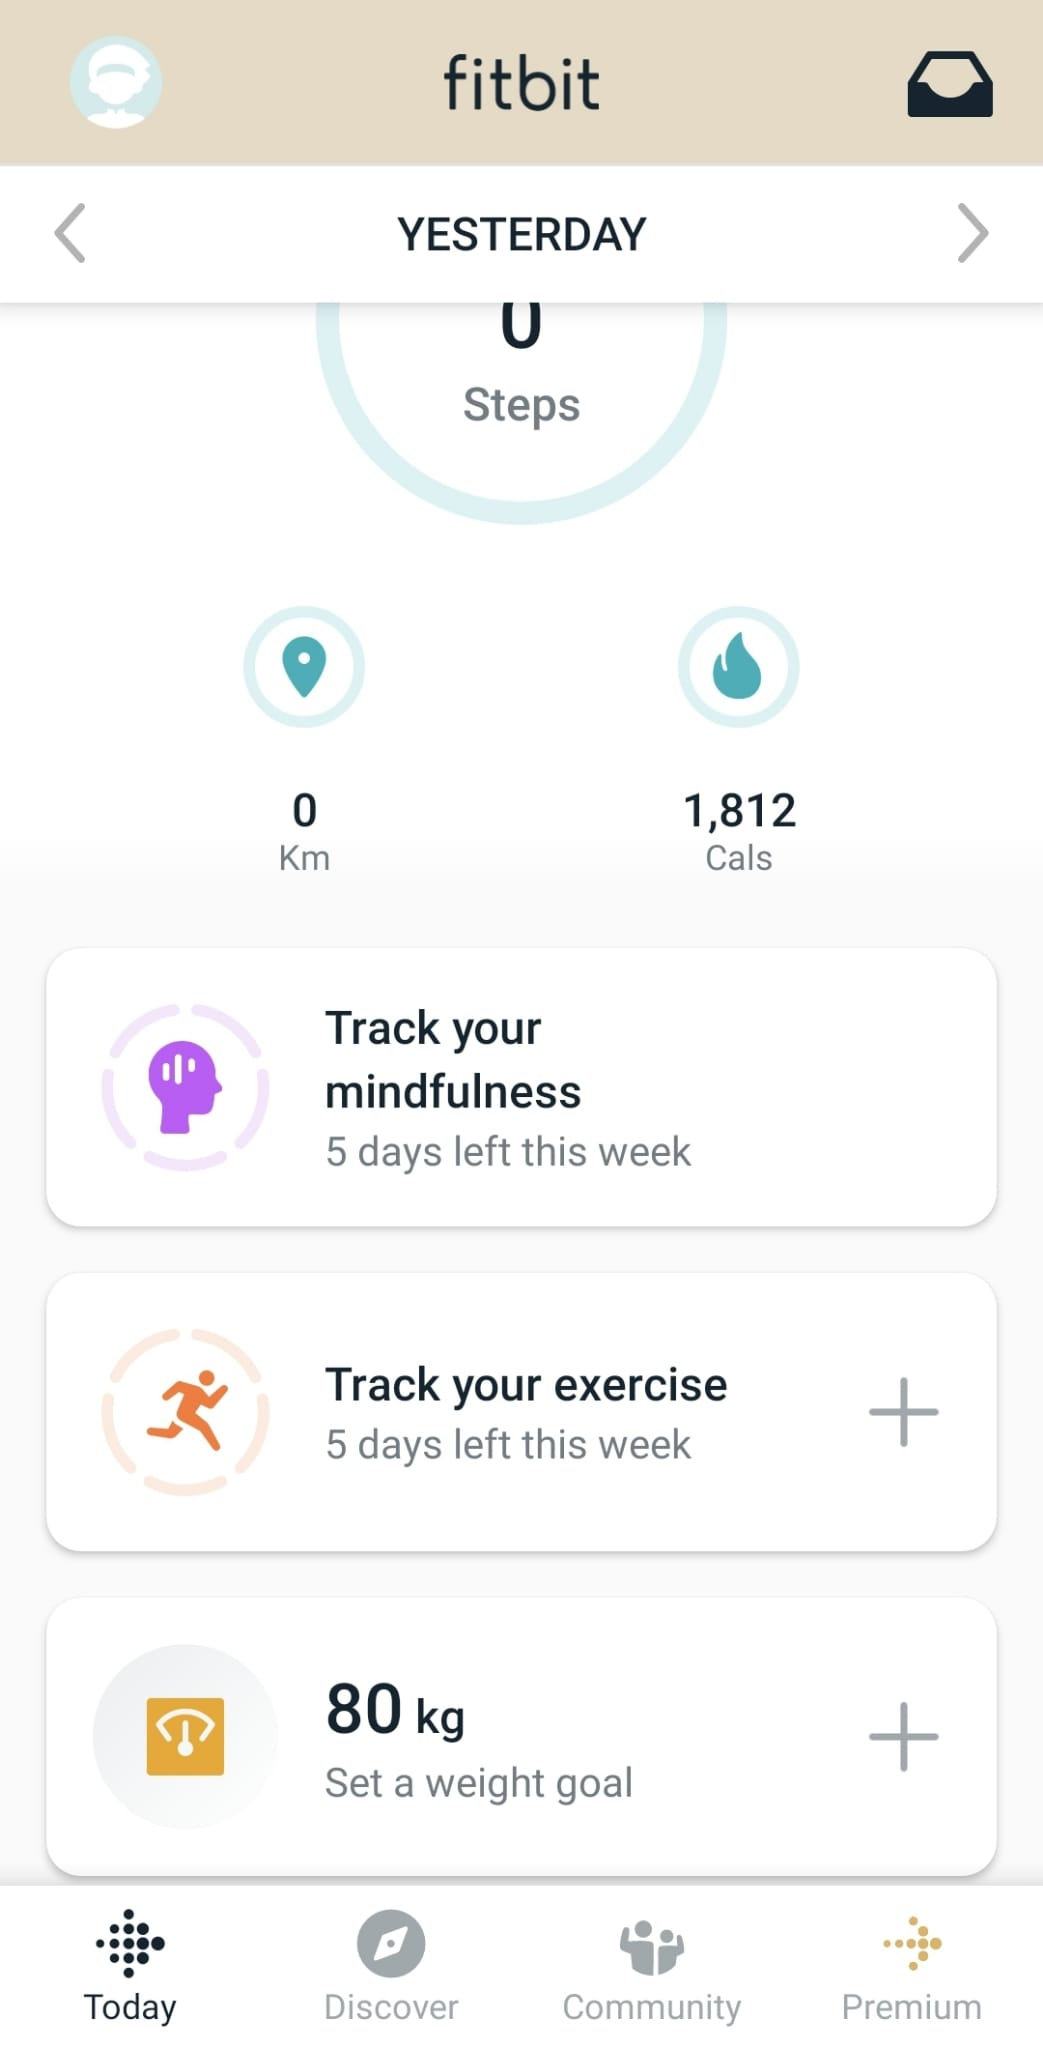
\includegraphics[width=0.5\textwidth]{fitbit/dashboard.jpeg}
        \caption{Dashboard}
        \label{fig:fitbit-home}
    \end{minipage}%
    \begin{minipage}{0.5\textwidth}
        \centering
        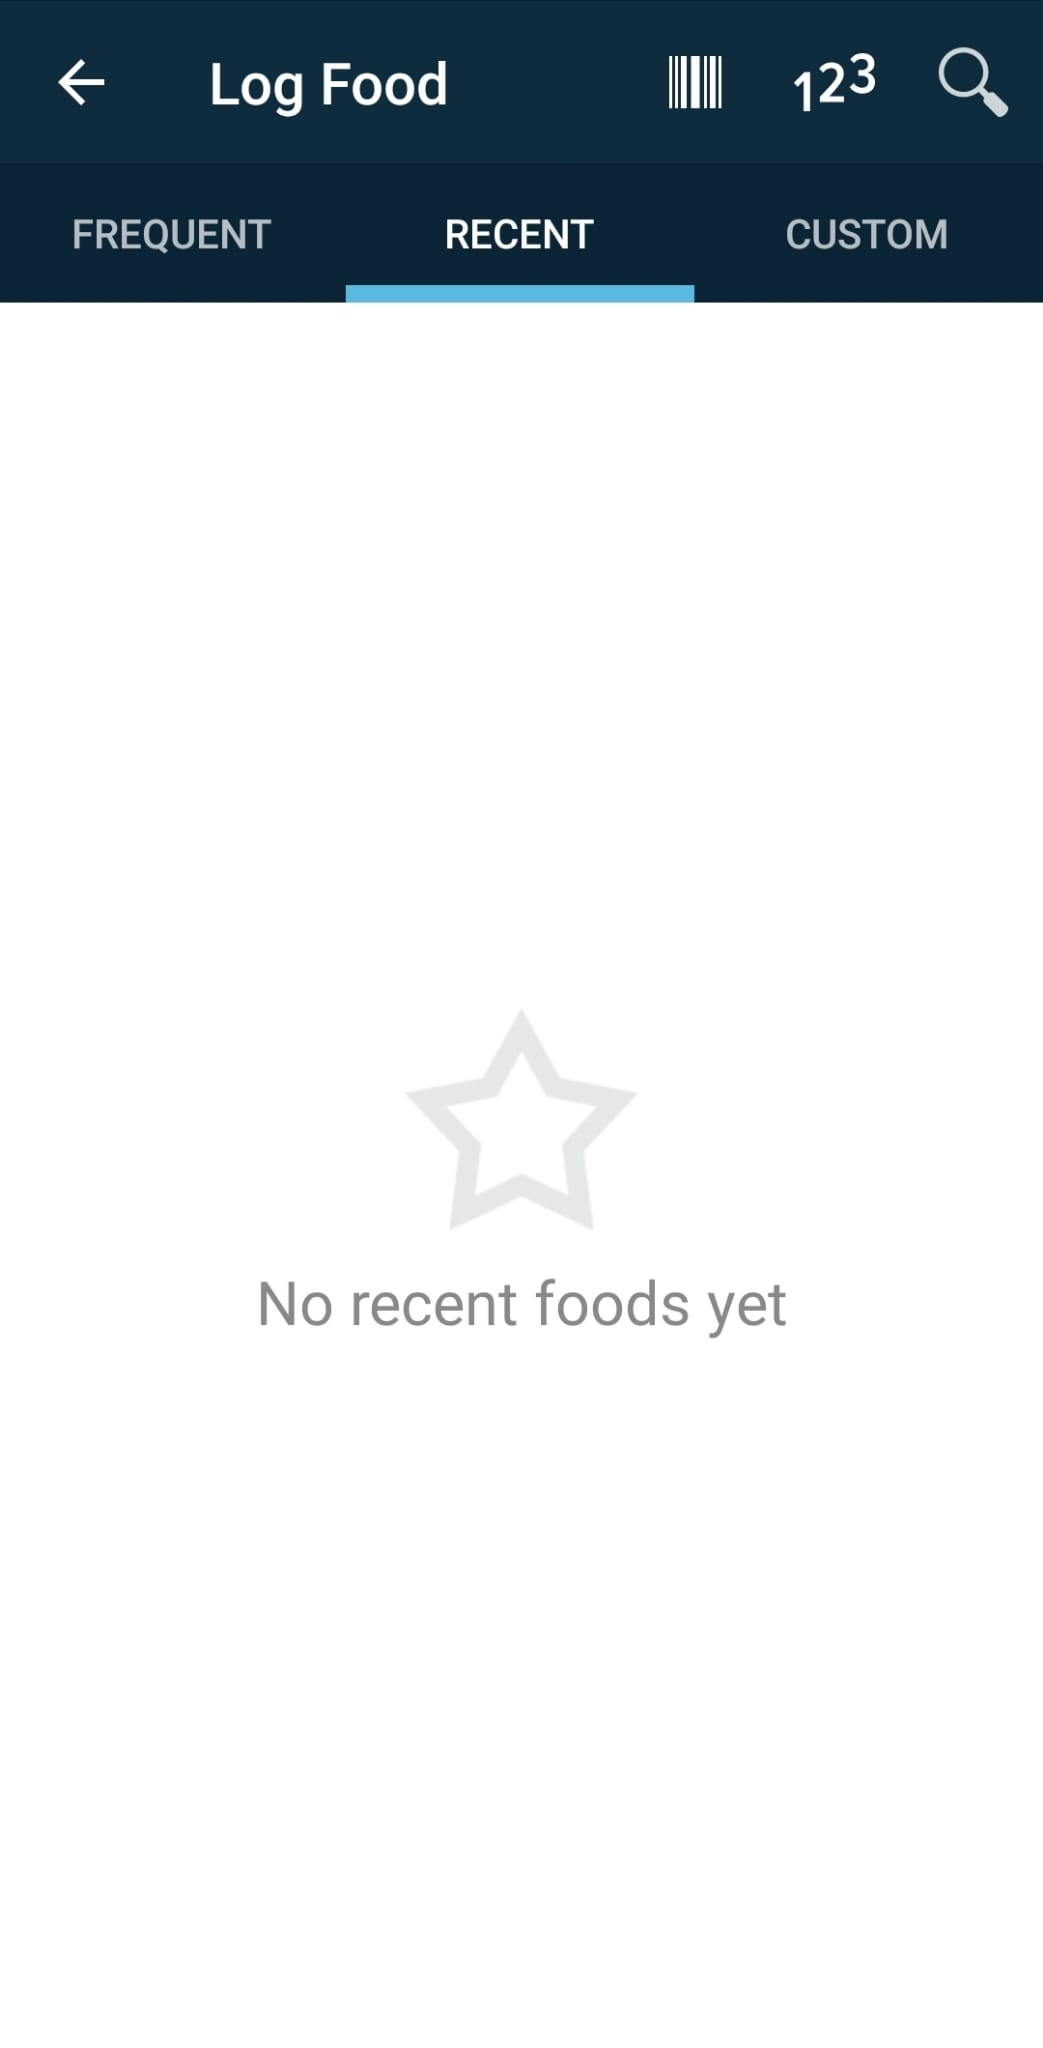
\includegraphics[width=0.5\textwidth]{fitbit/food-tracker.jpeg}
        \caption{Food log screen \& features}
        \label{fig:fitbit-log}
    \end{minipage}
\end{figure}
\textbf{User Story}
\label{research-breakdown:fitbit-usr-story}
\par
``As a professional athlete I wake up, go through guided meditation on my Fitbit calendar before weighing myself (\cref{fig:fitbit-home}).
I then log my breakfast and eat (\cref{fig:fitbit-log}), followed by my commute to practice
and logging my sport and duration (\cref{fig:fitbit-exercise-log}).''

\begin{figure}[H]
	\centering
	\includegraphics[width=0.25\textwidth]{fitbit/exercise-choice.jpeg}
	\caption{Using exercise search \& log}
	\label{fig:fitbit-exercise-log}
\end{figure}
\pagebreak


\textbf{Features/Functionality}
\label{research-breakdown:fitbit-features}
\par
Fibit includes all of the following features:
\begin{multicols}{2}
	\setlist{nolistsep}
	\begin{itemize}[noitemsep]
		\item Guided meditation (w/ simple week-calendar scheduling).
		\item Guided video workout plans (w/ simple week-calendar scheduling).
		\item Guided programmes (for meeting targets in health, not just fitness).
		\item Challenges (1-10 people, gamifying targets).
		\item Water tracking.
		\item Food tracking.
		\item Track exercise (only by sport/activity, no custom option and no individual exercises/routines).
		\item Step counter.
		\item Community feed and groups.
		\item Add friends and send/receive messages.
	\end{itemize}
\end{multicols}
\textbf{Technology Stack}
\label{research-breakdown:fitbit-stack}
\par
Fitbit uses the following technologies according to Stackshare \cite{fitbit-stack}:
\begin{itemize}
	\item JavaScript(and Ember.js) for the front end.
	\item Fastly (for cloud content delivery)
	\item Redis (for middle layer and database caching)
	\item Node.js (for producing backend APIs)
	\item Java (and Spring) for the non-mobile applications
	\item MySQL (for the backend database(s))
\end{itemize}
Fitbit is cross-platform and multifunctional, thus there will be some technologies
not in use by the mobile app we are researching. It's unlikely Spring
is in use, but the use of JavaScript (w/ Node.js) for the front and backend is
common in current world of software. It's highly likely
the whole system is using a microservice architecture where components maybe used in several places.
\pagebreak

\subsection{Comparing MyFitnessPal and Fitbit}
Firstly, we'll note that both applications make use of JavaScript for their front-end technologies.
It's difficult to pinpoint what is being used without decompiling both applications (both of which have a huge codebase).
It is apparent that MFP is using React\footnote{an open-source UI software framework created by Meta, Inc (formerly Facebook)}.
Both apps are also using some form of CDN to speed up content delivery, which is needed given the abundance of data involved in
the tracking of food and exercise. MFP offers developers access to their data set via their own API \cite{mfp-api}.
\par
Whilst both apps calculate calories burned (an arguably useless metric for \textit{our project})
during exercise, the scope and functionality of exercise is vastly different.
Fitbit includes general sports and activities but no specific exercises (for example
- ``weights'' is considered 1 exercise type and the calories burned are dependent on duration)
and there is no ability
to produce your own routine.
On the other hand, MFP allows for the creation (and sharing) of your own routines using their
database of exercises. There are no videos to follow for this component of the app.
Both apps do however offer workout routines (and short-term programmes) via 
short videos published by the respective companies.
\par
Both apps allow for the tracking of food and water intake, as well as the ability
to scan product barcodes to log nutritional information. In regard to overall wellness,
Fitbit seems to be covering more ``bases'' by providing guided meditation videos and challenges
which can be taken alone or as a group. These challenges are a way to gamify the achievement of
personal goals (such as using your phone less).
\par
Finally, both apps include community features - very similar to traditional social media platforms.
These and other nutrition focused features are beyond the desired scope of \textit{our project} (\cref{chap:project-specification}) thus we won't be
comparing and considering these.
\par
Overall, the fitness aspect of MFP seems more useful, but there are elements of the app which are not yet
on par with Fitbit - such as the goal setting and mindfulness measurements. 
That said, the UX/UI of MFP is more usable and the app has fewer features locked behind hardware devices
(yet you can still pair compatible devices to MFP). Neither app has any major feature involving the camera besides
the barcode scanning components. A combination of elements from both apps will be paramount to a successful project.
\par

\textit{The project} is planned to have a side panel 
menu and similar minimal aesthetic to that of MFP (\cref{sec:UI-design}).
It's not planned that it will include the calories burned estimates; however other metrics will be included in similar vain, such
as total time trained and cumulative weight lifted/cumulative distance travelled. Calorie estimates will be an enhancement (additional feature) where time permits.
The abilities to create custom routines and follow preset routines, which are featured in MFP and Fitbit respectively,
are expected to be important features in \textit{the project}. Albeit, the long term plan
is to support the ability for trainers to set these programmes as opposed to presets alone. 
\par
In summary, the design
and layout of these apps is what's useful for us - inspiration and additional features can also be drawn
from these existing systems. With that said, \textit{our product} is not a nutrition tracker and focusing
on elements in this space would shift the scope of the \textit{project} substantially (\cref{risk:mitigation-scope}). An extensive
breakdown of the feature set can be found in \cref{sec:features}.
\pagebreak
\subsection{TrueCoach}
TrueCoach provide a cross-platform system that includes a web application.
We'll be considering the mobile app provided for end users and making reference
to the functions available to administrators in the process. They provide a mobile app
for each of these use cases - ``\textbf{TrueCoach for Clients}'' and ``TrueCoach Connect'' for trainers.
\begin{figure}[H]
	\centering
	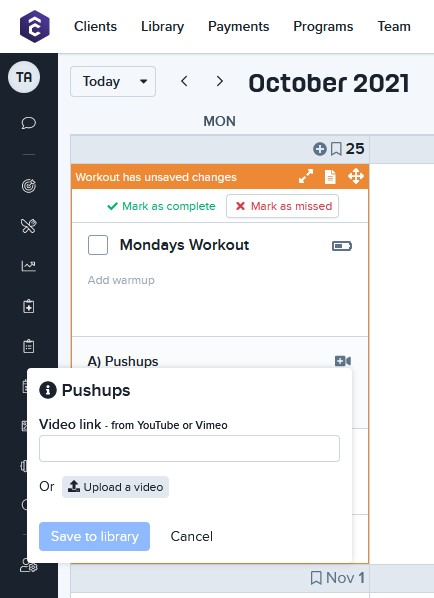
\includegraphics[width=0.3\linewidth]{truecoach/setting-client-workout.jpg}
	\caption{Trainer using web app to set clients workout(s).}
	\vspace*{-5mm}
	\label{fig:tc-trainer-set}
\end{figure}
\begin{figure}[H]
	\centering
	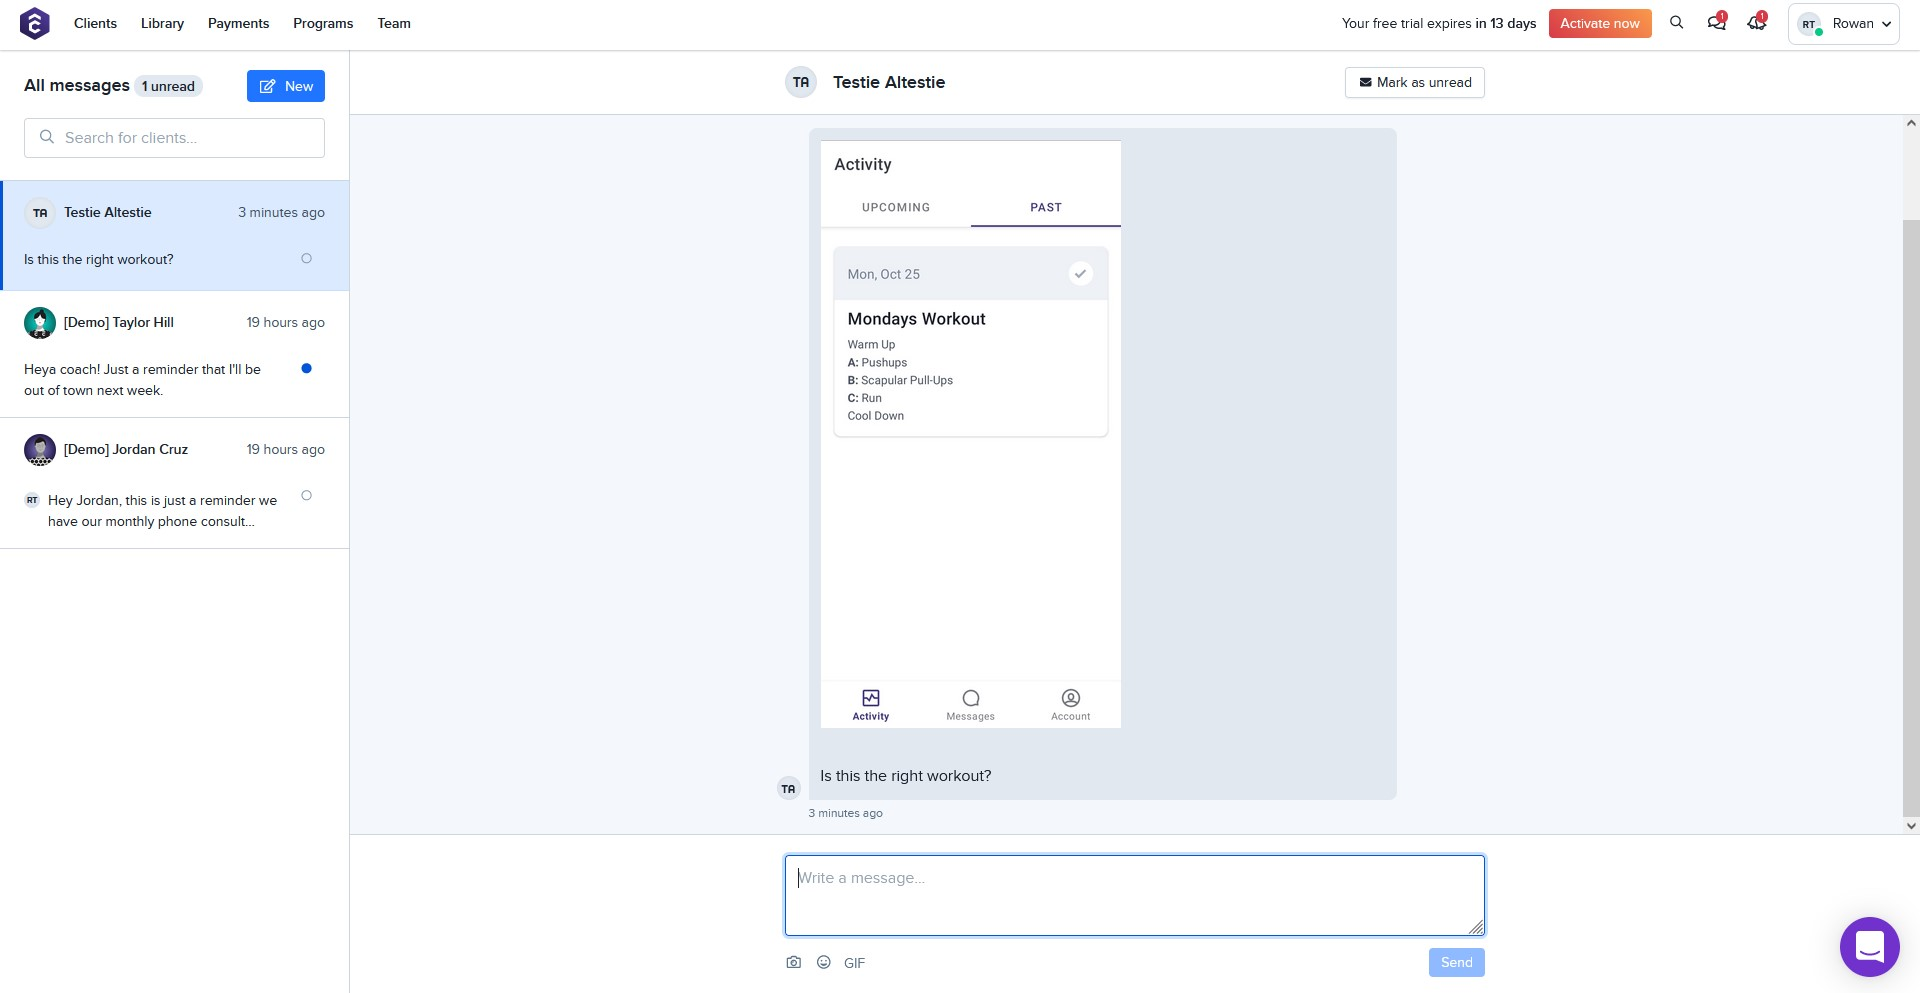
\includegraphics[width=1\linewidth]{truecoach/truecoach-web-chat.jpg}
	\caption{Trainer using web chat to manage clients.}
	\vspace*{-5mm}
	\label{fig:tc-trainer-chat}
\end{figure}
\textbf{User Story}
\label{research-breakdown:tc-usr-story}
\par
``As a new gym go-er, I work remotely with my trainer (\cref{fig:tc-trainer-chat,fig:tc-user-chat}) to refine my training technique(s).
I view my upcoming workouts (\cref{fig:tc-activity}) and follow instructional videos before marking my workouts as complete and monitoring 
my progress via goals \& challenges (\cref{fig:tc-workout}). For advice I can view
documents and progress photos in my settings page (\cref{fig:tc-settings}).''
\begin{figure}[H]
    \centering
    \begin{minipage}{0.4\textwidth}
        \centering
        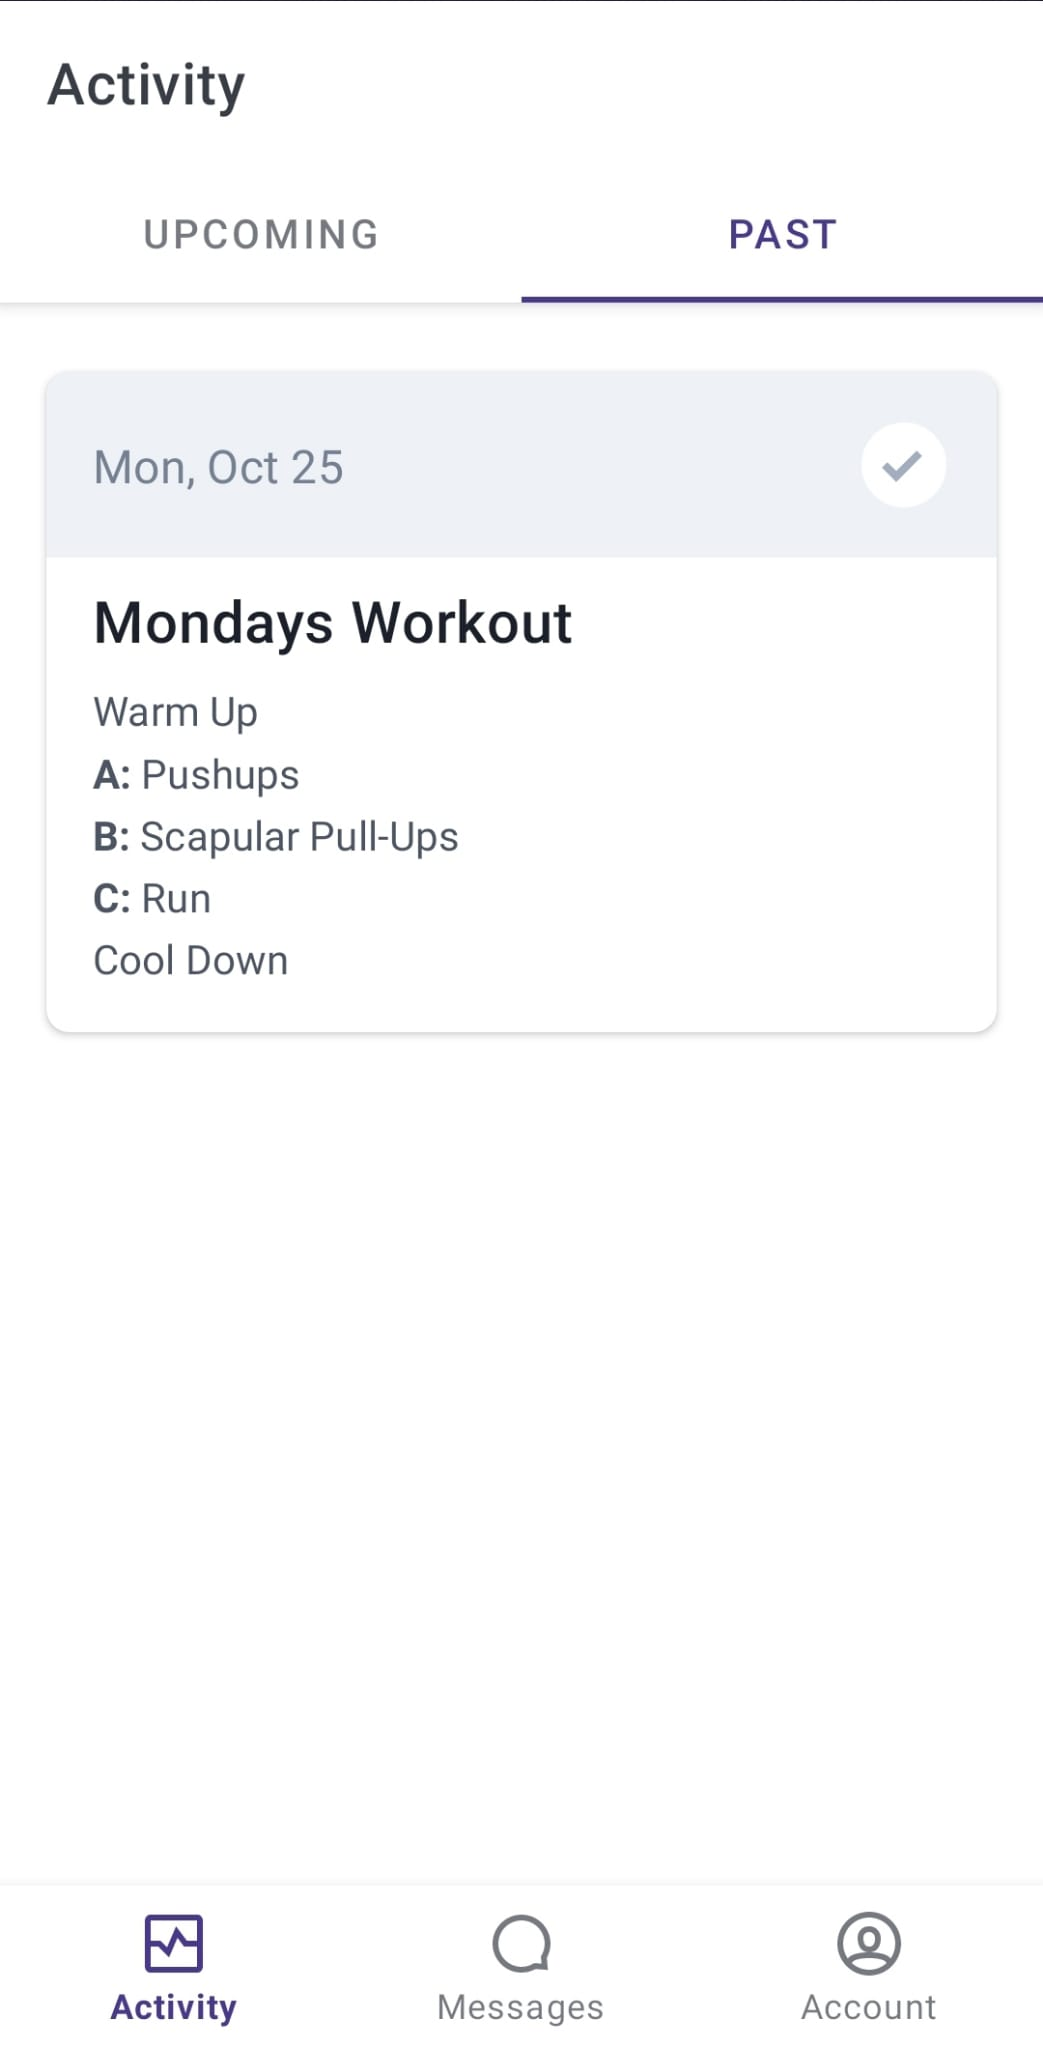
\includegraphics[width=0.5\linewidth]{truecoach/activity-page.jpeg}
        \caption{Viewing workouts (upcoming/past).}
        \label{fig:tc-activity}
    \end{minipage}\qquad
    \begin{minipage}{0.4\textwidth}
        \centering
        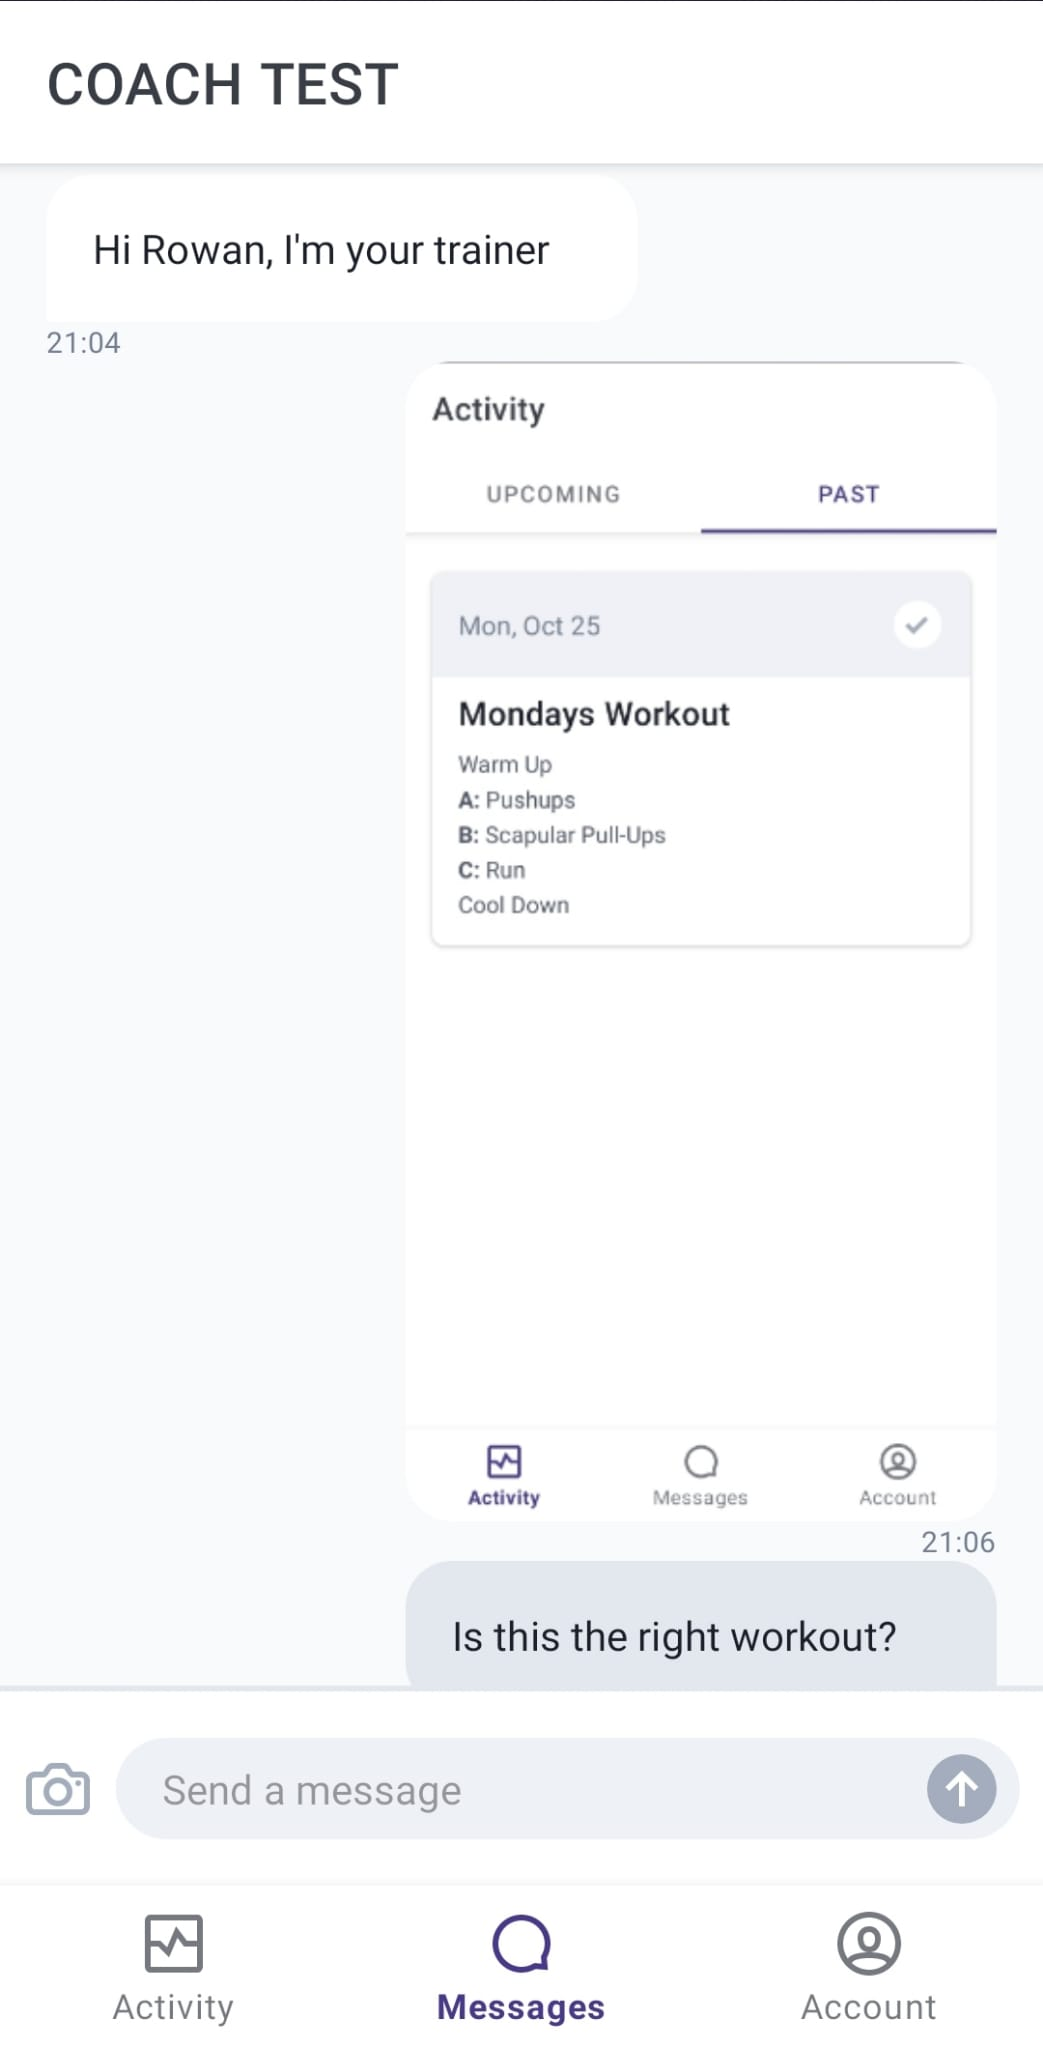
\includegraphics[width=0.5\linewidth]{truecoach/trainer-chat.jpeg}
        \caption{Instant messaging with a trainer.}
        \label{fig:tc-user-chat}
    \end{minipage}%
\end{figure}
\vspace*{-5mm}
\begin{figure}[H]
    \centering
    \begin{minipage}{0.4\textwidth}
        \centering
        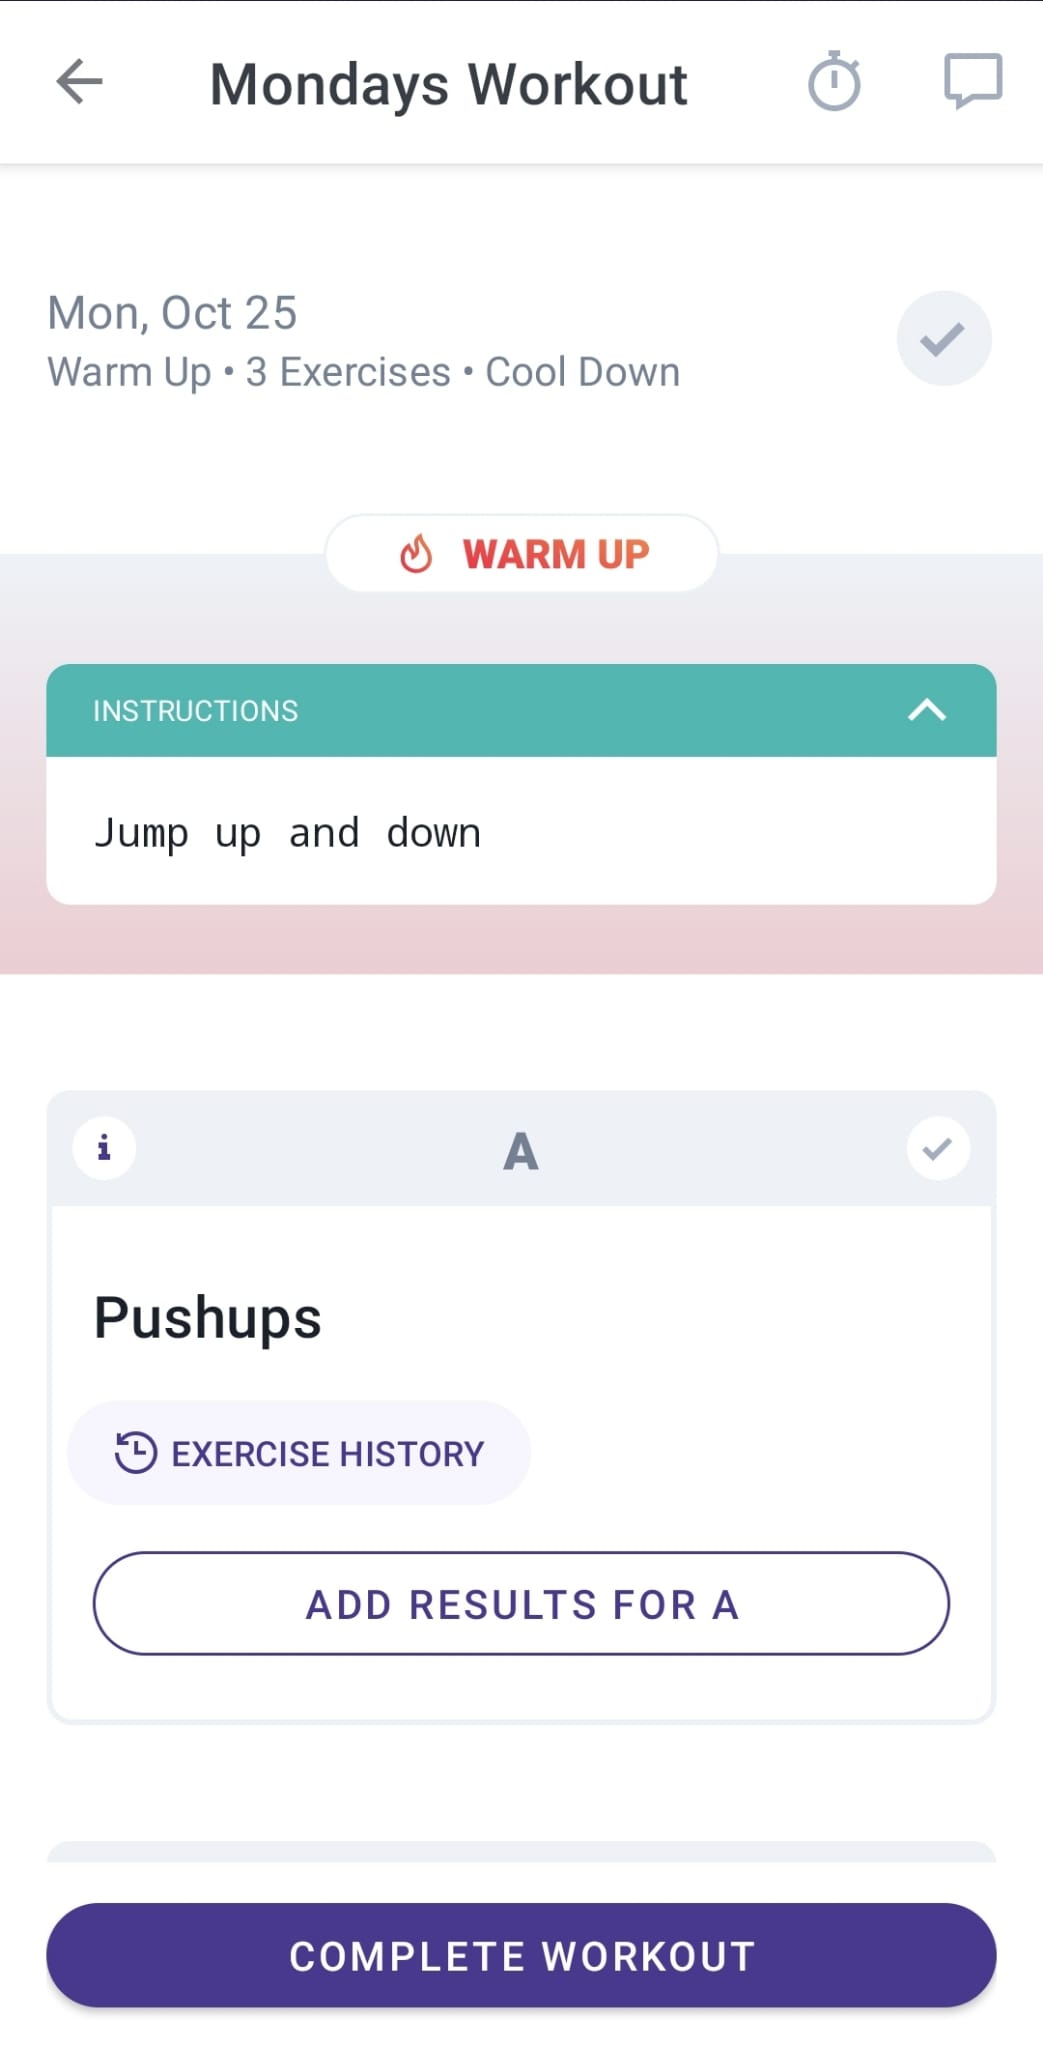
\includegraphics[width=0.5\linewidth]{truecoach/workout-logging.jpeg}
        \caption{Logging a workout.}
        \label{fig:tc-workout}
    \end{minipage}\qquad
    \begin{minipage}{0.4\textwidth}
        \centering
        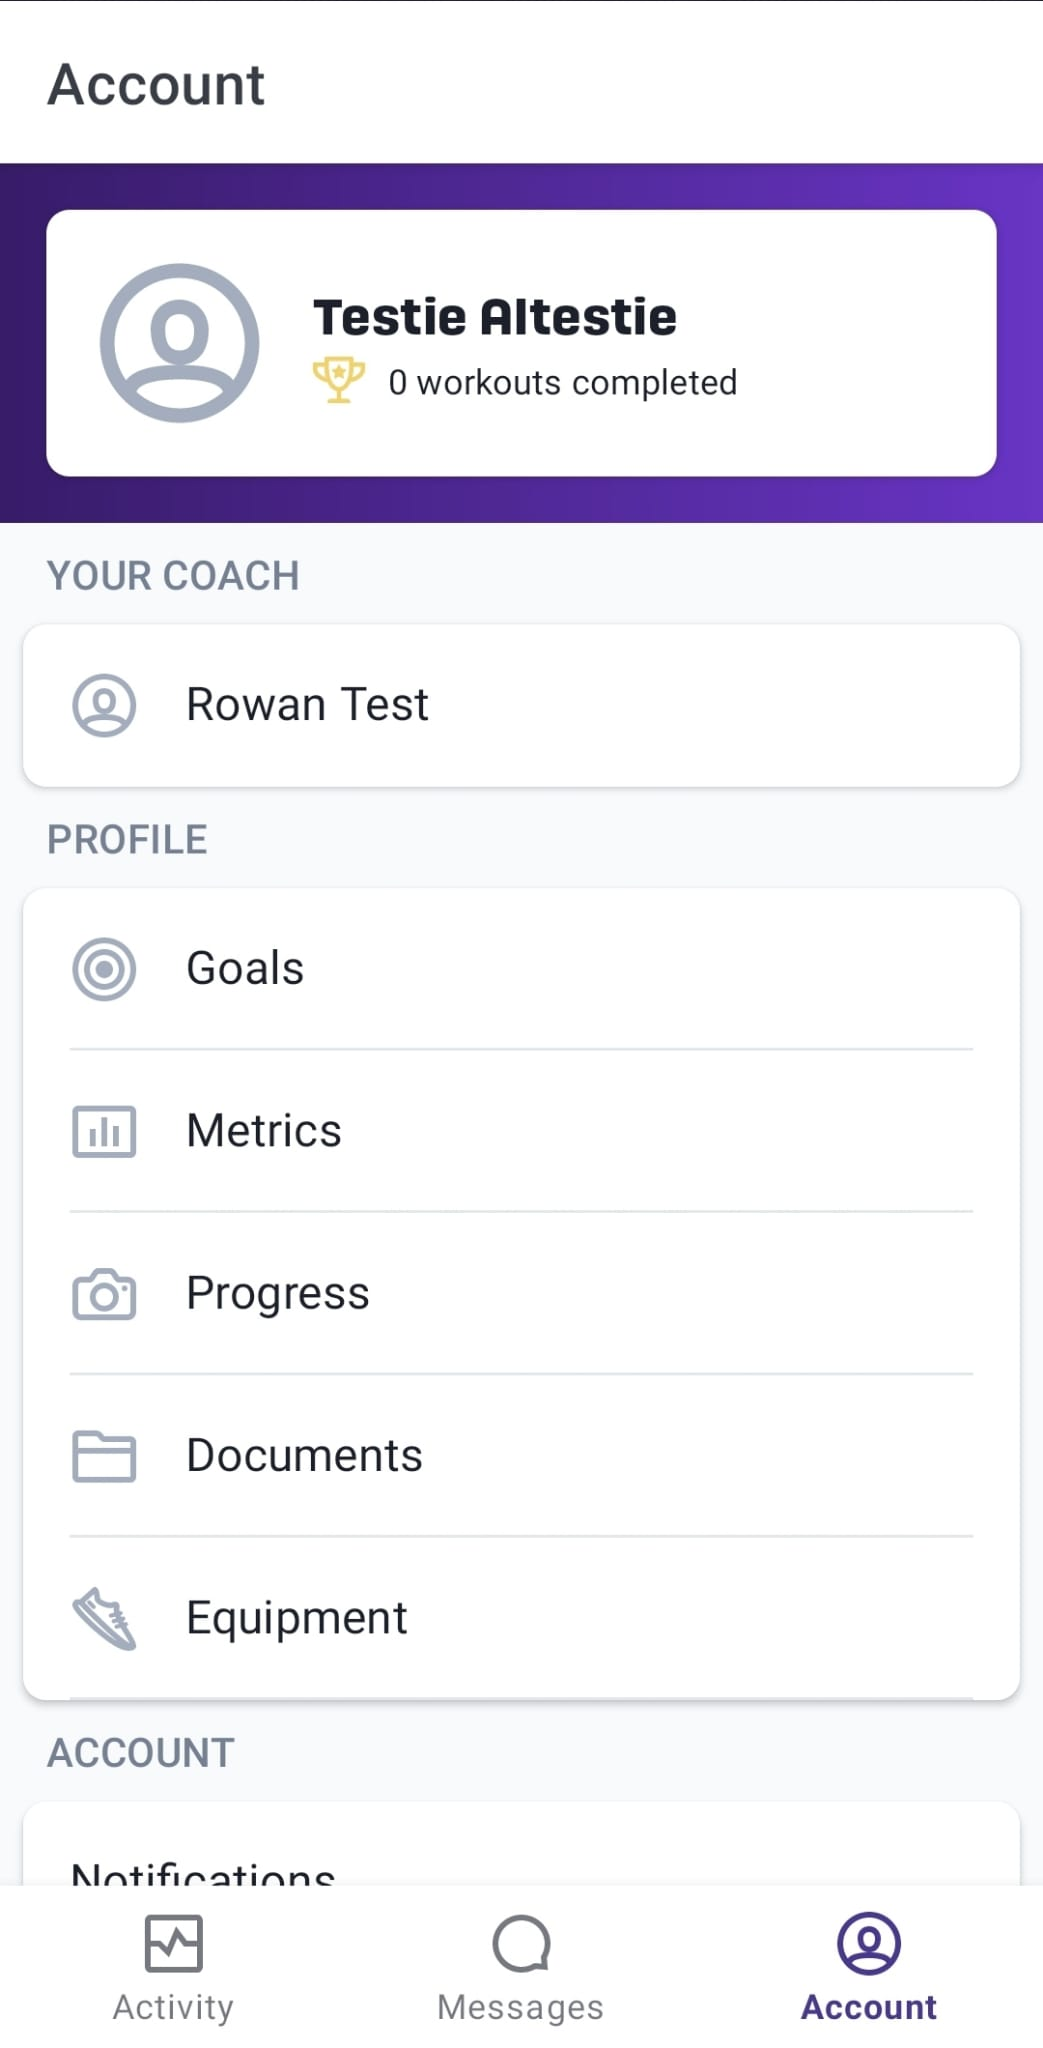
\includegraphics[width=0.5\linewidth]{truecoach/settings.jpeg}
        \caption{Viewing settings.}
        \label{fig:tc-settings}
    \end{minipage}%
\end{figure}
Above, ``Testie Altestie'' represents an end user and ``Rowan Test'' is the trainer. We can see
the functions available to the user are dependent on the workouts uploaded/scheduled
by the trainer using their interface (web application in this case).
\pagebreak

\textbf{Features/Functionality}
\label{research-breakdown:tc-features}
\par
\textbf{``TrueCoach for Clients''} includes all of the following features:
\begin{multicols}{2}
	\setlist{nolistsep}
	\begin{itemize}[noitemsep]
		\item Track coach's release of phased training (upcoming/past workouts).
		\item Log workouts (w/ notes).
		\item Timer \& stopwatch function for tracking timed exercises.
		\item Video breakdowns of exercises (w/ rich text instructions).
		\item Instant messaging w/ trainer (including multimedia uploads).
		\item Tracking of progress via trainer-set goals \& metrics.
		\item Progress and additional documents (outbound link to web app).
		\item Create account via invite link from trainer.
		\item View notifications.
		\item Edit settings (outbound link to web app).
	\end{itemize}
\end{multicols}
\vspace*{-5mm}
TrueCoach covers a lot of needs for a user, and we can see in \cref{fig:tc-trainer-chat} 
the relevant tools for the trainer to facilitate these workouts. They are administrators of their
clients and they're the means by which a user gets login credentials. 
Trainers can upload relevant videos (\cref{fig:tc-trainer-set}) and documents, as well as provide metrics
to measure users progress.
\par
\textbf{Technology Stack}
\label{research-breakdown:tc-stack}
\par
Stackshare (as used for the previous apps) is not useful in this case, so the following conclusions have
been drawn following the decompilation of the TrueCoach APK \cite{apk-decompiler}:
\setlist{nolistsep}
\begin{itemize}
	\item Kotlin \& Java (for Android development)
	\item Firebase (for push notifications and messaging)
	\item AWS Amplify (for backend deployment)
	\item Numerous open-source development packages such as \href{https://github.com/bumptech/glide}{glide}. 
\end{itemize}
After decompiling and opening the class files using \href{https://github.com/pxb1988/dex2jar}{dex2jar} and
\href{https://java-decompiler.github.io/}{JD-GUI}, I found that the application is not using a cross-platform
JavaScript framework as is standard in modern times. The app is using the recommended native language
of Kotlin\footnote{Learn more: \href{https://developer.android.com/kotlin}{android development documentation}} and Java for all data objects and frontend display. 
\pagebreak

\subsection{Exercise.com}
Exercise.com are the company providing the white-labelled solution behind \href{https://online.pjfperformance.net/users/sign_in/}{PJFPerformance}.
We'll be using the \textbf{PJFPerformance} app to analyse their application.
\begin{figure}[H]
    \centering
    \begin{minipage}{0.5\textwidth}
        \centering
        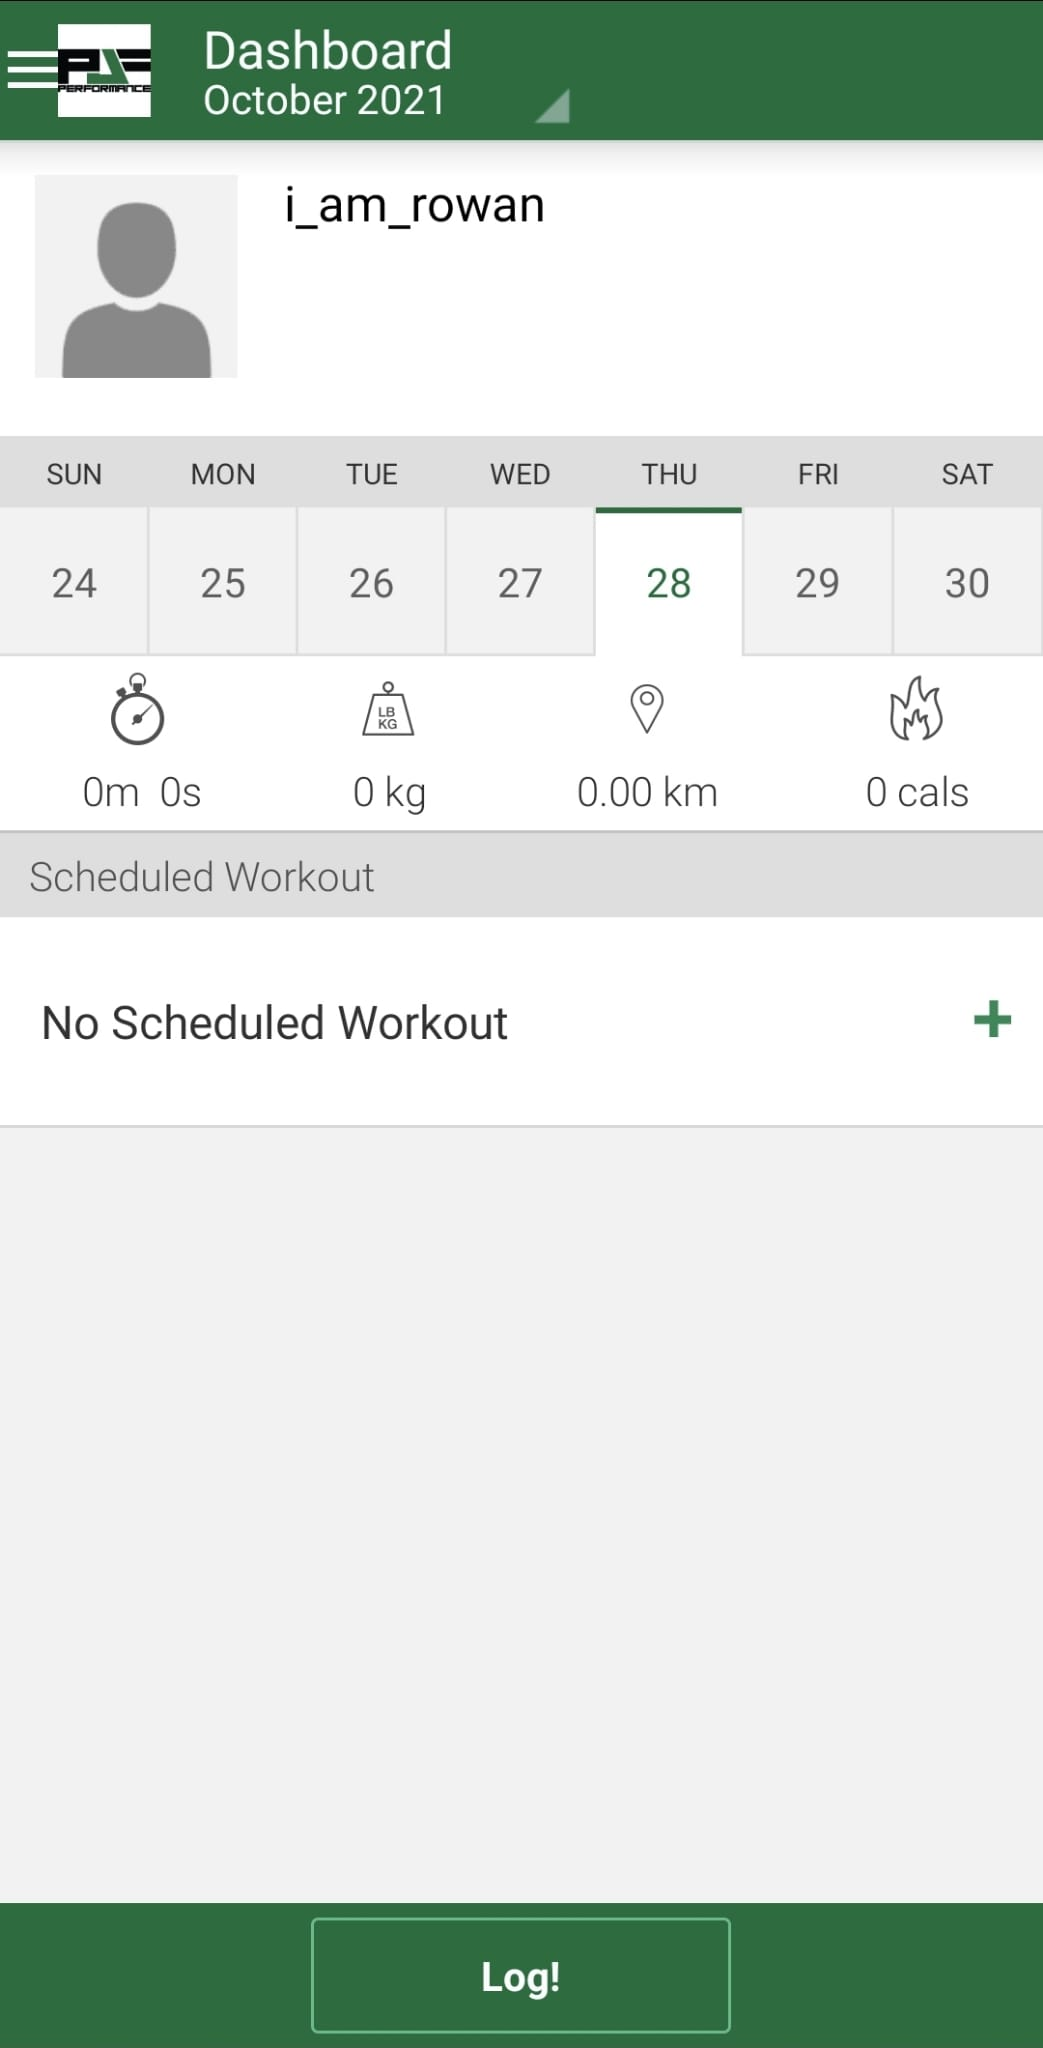
\includegraphics[width=0.5\textwidth]{pjf/pjf-dashboard.jpeg}
        \caption{Home dashboard}
        \label{fig:pjf-home}
    \end{minipage}%
    \begin{minipage}{0.5\textwidth}
        \centering
        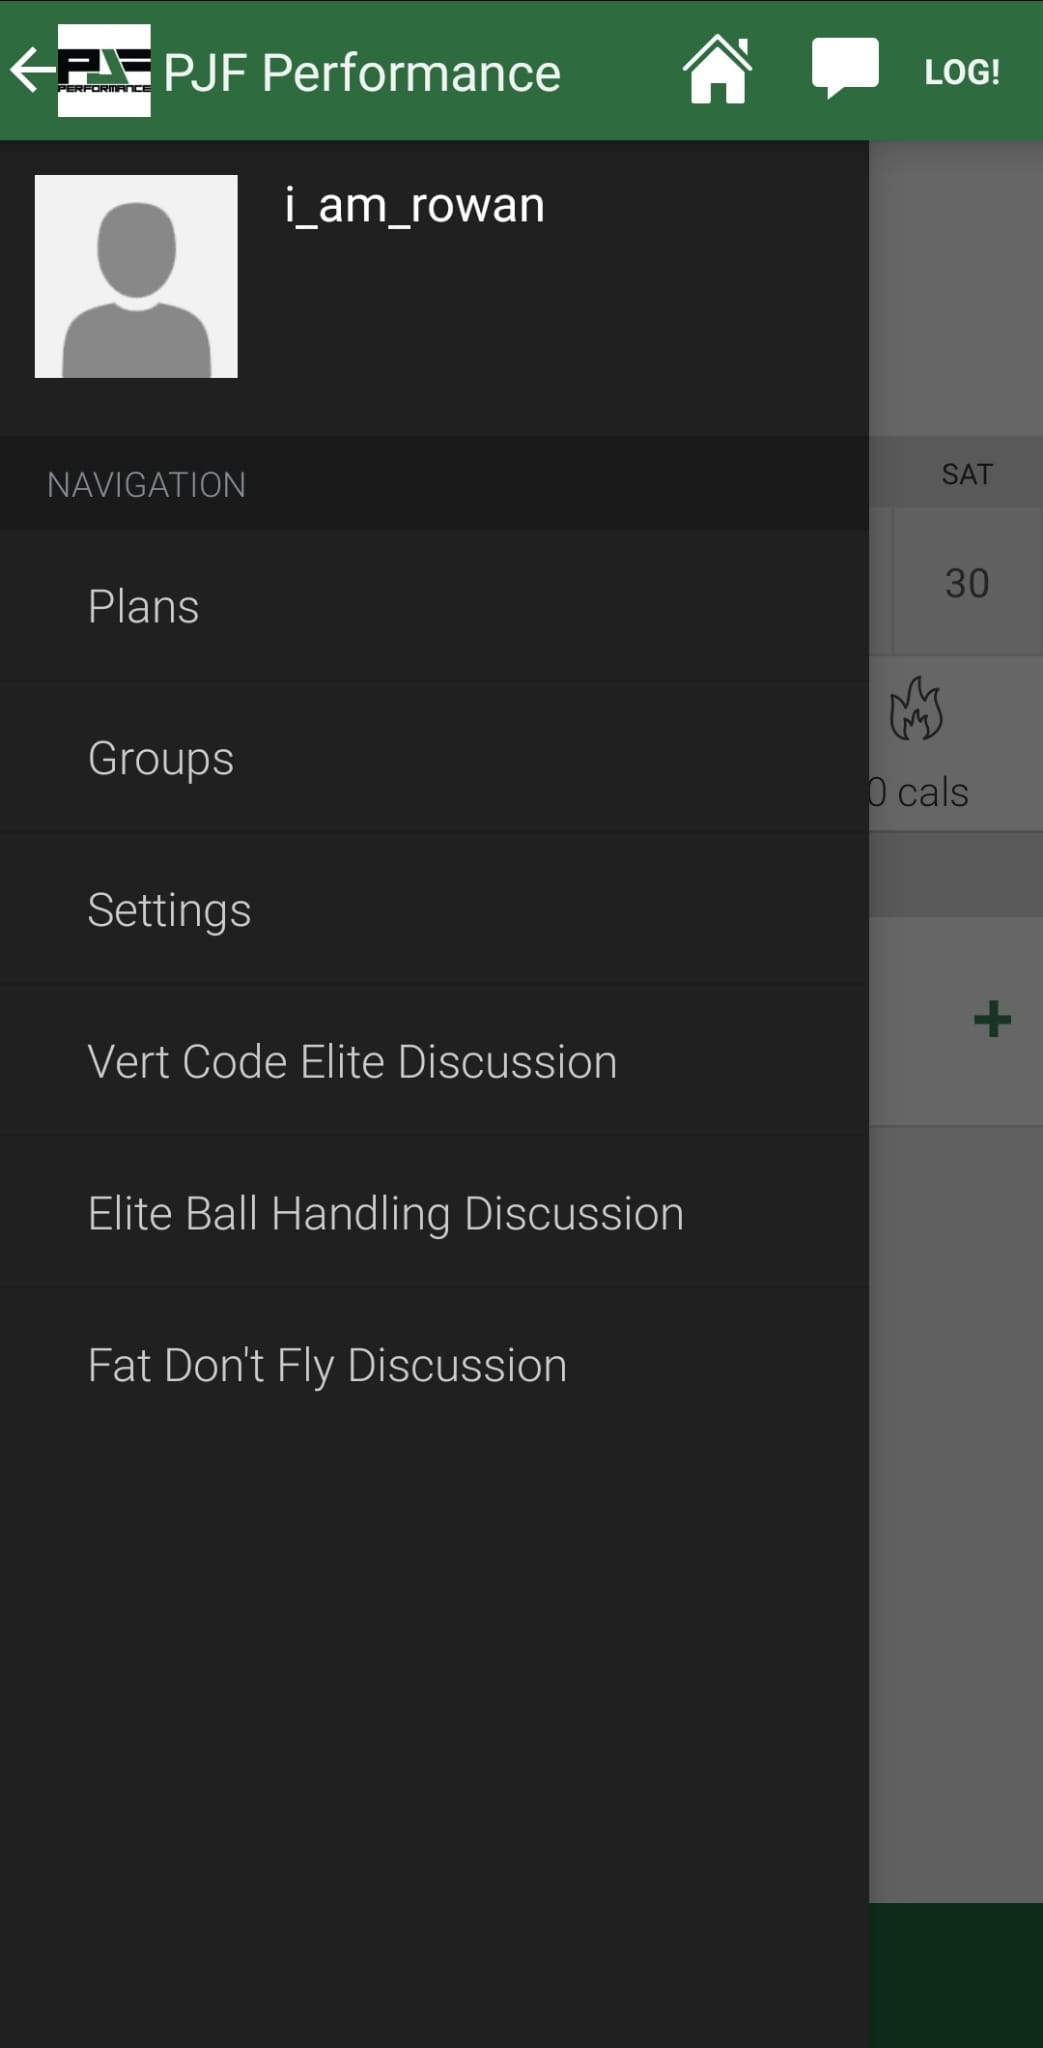
\includegraphics[width=0.5\textwidth]{pjf/pjf-menu.jpeg}
        \caption{Sidebar menu options}
        \label{fig:pjf-menu}
    \end{minipage}%
\end{figure}
\begin{figure}[H]
    \centering
    \begin{minipage}{0.5\textwidth}
        \centering
        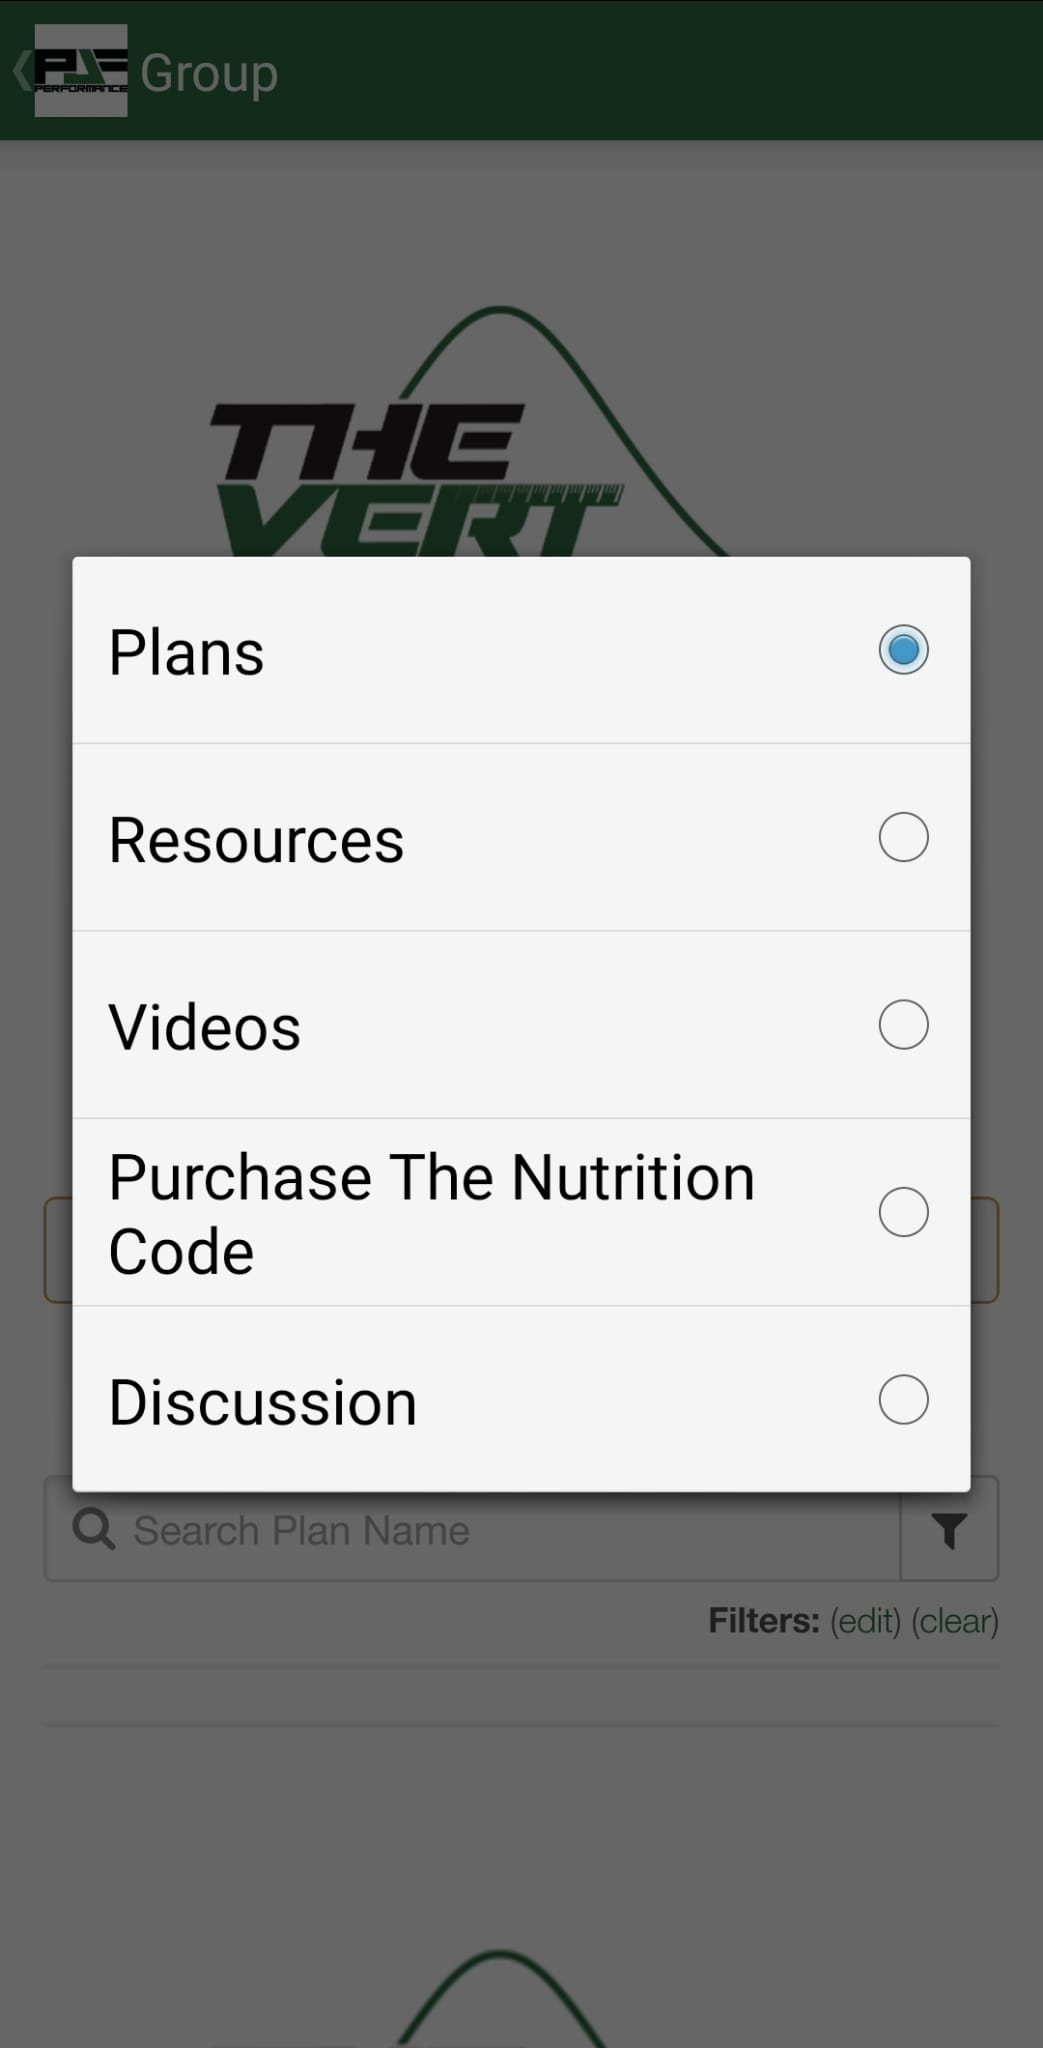
\includegraphics[width=0.5\textwidth]{pjf/pjf-group-resources.jpeg}
        \caption{Viewing additional resources.}
        \label{fig:pjf-resources}
    \end{minipage}%
    \begin{minipage}{0.5\textwidth}
        \centering
        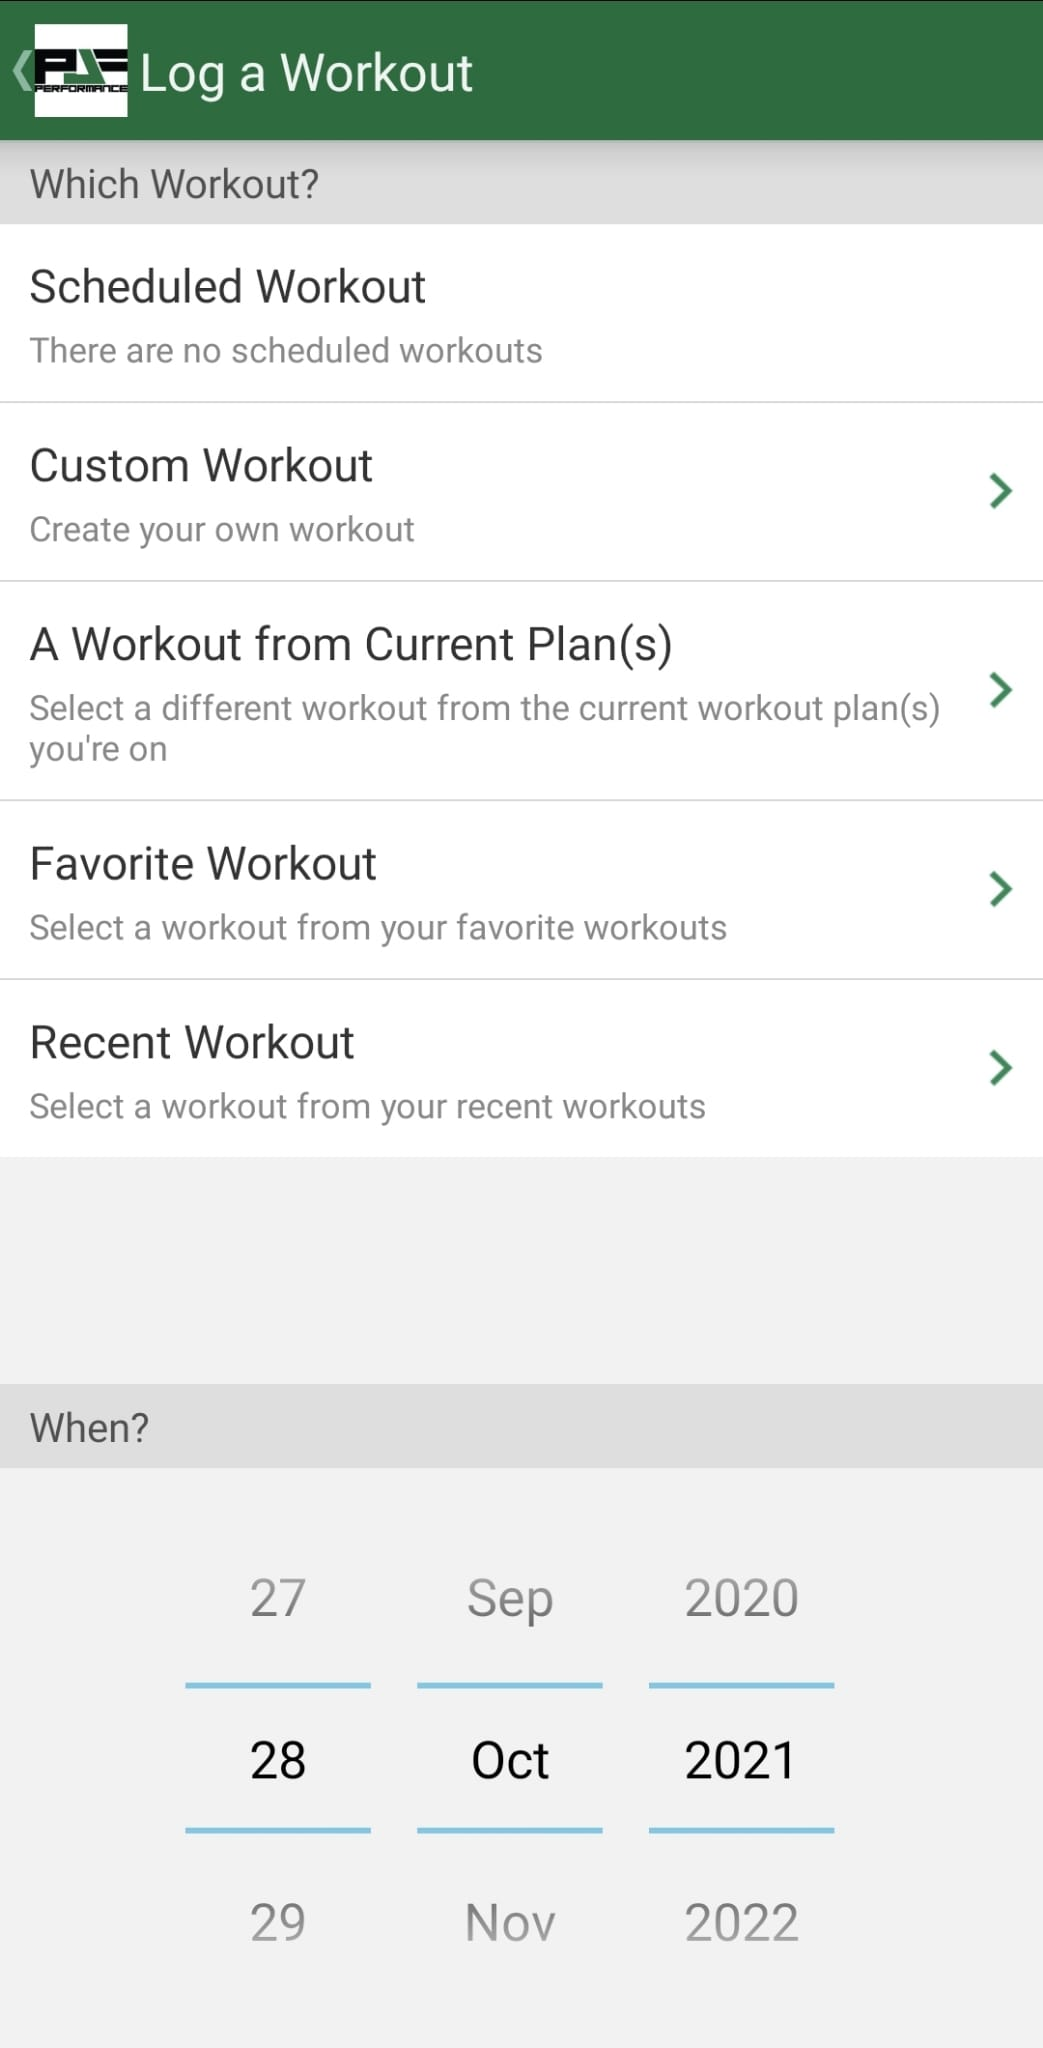
\includegraphics[width=0.5\textwidth]{pjf/pjf-logging-workout.jpeg}
        \caption{Scheduling/logging a workout.}
        \label{fig:pjf-workout}
    \end{minipage}%
\end{figure}
\pagebreak
\textbf{User Story}
\label{research-breakdown:pjf-usr-story}
\par
``As a basketball player, I enroll to Paul Fabritz' workout plan using the web application before
receiving credentials for the mobile app. Here I schedule the programme to begin
at the start of the month and I allocate days of the week for my workouts (\cref{fig:pjf-home}).
I create my profile containing my weight and other metrics, so I can ask relevant questions
to Paul and others on the same programme as me via a discussion room (\cref{fig:pjf-menu}). For guidance on training
during the season and managing load, there is a resources section (\cref{fig:pjf-resources}) (outbound links). I log all my workouts and make notes
for my own use. I sometimes create workouts for myself (\cref{fig:pjf-workout}) using some exercises available through the app.
Whenever I train, I can see exercises explained via videos embedded from YouTube.''

\textbf{Features/Functionality}
\label{research-breakdown:pjf-features}
\par
The PJFPerformance app includes all of the following features:
\begin{multicols}{2}
	\setlist{nolistsep}
	\begin{itemize}[noitemsep]
		\item Schedule workouts.
		\item Create custom workouts (using existing exercises).
		\item Log workouts (w/ notes).
		\item Enroll on phased programmes (made up of multiple workouts split over
		a given number of weeks \& days).
		\item Edit profile.
		\item View settings.
		\item View notifications.
		\item Rest timer for timed sets in workouts.
		\item Videos (YouTube hosted) for exercises.
		\item Group discussions for programmes.
		\item View additional resources (hosted externally).
	\end{itemize}
\end{multicols}
\vspace*{-5mm}
Exercise.com work on a 1-to-1 basis with trainers and white-label their solutions, this means
any administrator view can only be presumed via the decompilation of the APK app file.

\textbf{Technology Stack}
\label{research-breakdown:pjf-stack}
\par
Similarly to \hyperref[research-breakdown:tc-stack]{TrueCoach}, finding the technology used by Exercise.com for the mobile application is only possible
via decompilation using existing tools \cite{apk-decompiler}.
Based on my look into the source code, we can safely conclude that the app uses:
\setlist{nolistsep}
\begin{itemize}
	\item Kotlin \& Java (for Android development)
	\item Firebase (for push notifications and messaging)
	\pagebreak
	\item Amazon S3 (for data storage)
	\begin{itemize}
		\item They expose data from the S3 instance via their web application API.
		This is where the mobile application is pulling data from.
		\item The S3 instance  is using some form of SQL database (we know this based on SQL migration scripts in the source code).
	\end{itemize}
	\item Numerous open-source development packages such as \href{https://github.com/alibaba/fastjson}{FastJson}. 
\end{itemize}
Similarly to \hyperref[research-breakdown:tc-stack]{TrueCoach}
this app is written using Kotlin and not a cross-platform JavaScript framework.
The MaterialDesign\footnote{a design language invented by Google (Android parent company) in 2014.}
influence is noticeable in this app and so it is less surprising. Performance to the User
feels somewhere between average and slow for this type of app.

\subsection{Comparing TrueCoach and PJFPerformance (Exercise.com)}
TrueCoach has a larger focus on the client-trainer relationship and is more suited to
the public (anybody can become an administrator and begin using their platform for their business).
On the other hand, PJF provides a greater reliance on the community of people following the same 
programme as the User. Our project aims to blend both of these concepts; the core functionality will be developed first (focusing on the end user)
before producing administrator views and allowing a many-to-many relationship between clients and trainers.
\par
From a technical standpoint the implementation of the applications are similar (both using Kotlin and Java, with
some use of open-source packages for specific needs - such as confetti in TrueCoach when completing a challenge).
Both apps also make use of Firebase messaging for push notifications. This is easily implemented
and simplifies the implementation of push notifications across platforms (Android/iOS). This is noteworthy for
the development of our project and will prove useful if Firebase is used instead of or alongside the technologies outlined
in \cref{sec:tech-stack}. Our application frontend will be built
using Flutter. The reasoning for this will be outlined further in the document, but performance is not expected to be adversely affected.
Whilst the technology will be different the functionality and user experience aims to be similar to that of both apps.
\par
TrueCoach has a simple 3 screens - logging and monitoring workouts (\cref{fig:tc-workout}) has a much better UX/UI.
The ability for a trainer to add new exercises and accompanying video
 (both via embeds or uploading raw video) is unique (\cref{fig:tc-trainer-set}). These are features that are
greatly beneficial to our project and reducing the number of app screens and keeping the interface minimal will
both provide a much better final product and ease the time stress of development and testing.
Only in the PJF app can a user create their own workout and log this (\cref{fig:pjf-workout}). This ability is
core to our app. On the other hand, the TrueCoach app is entirely dependent
on a trainer/administrator supporting you throughout your programme. Furthermore,
TrueCoach allows for the measurement of set metrics (by the trainer) and goals to surpass.
The PJF app lacks these features but does allow for further planning in the form of a calendar view and 
a ``traffic-light system'' for workouts on a daily basis. A red circle appears under missed workouts
on the calendar, amber for pending workouts for the day and green for completed workouts. TrueCoach
has personal goals but no extensive calendar view and there is a simple ``mark as completed'' feature
for scheduled workouts. We plan for both of these elements
to be included in our project; looking at the preliminary
prototype (\cref{fig:prototype}) and feature set (\cref{sec:features}) should provide more clarity on how this will be achieved.
\par
The final difference I consider notable between the apps is the use of timers. TrueCoach makes use of both
a stopwatch and a timer for users to utilise during exercises. Alternatively, PJF includes a rest timer
which Paul suggests to use for other functions but no stopwatch if needed (for example, when training for speed).
We plan on following TrueCoach's example here and allowing users the option of both. Implementation is relatively easy
 and should enhance user experience.
\par 
Many of the differences outlined above come down to the business objectives of the relative applications. TrueCoach is building a
SaaS company whereas Exercise.com is building a fitness application product that they can
white-label to notable trainers in the fitness industry. This core difference means there are certain
design decisions that differ between the apps. A common and core feature with both is the 
ability for users to view videos of exercises during workouts and to log there progress as they exercise.
This is important to the success of \textit{the product} and the approach we are looking at following involves
a dashboard upon registration where a trainer can include their branding and thereby personalise the end user
experience - similar to Stripe (\cref{fig:stripe-customization}).
\pagebreak

This functionality falls beyond the scope
of the outlined \textit{project} but will help you form a long-term understanding of the proposed system.
\par
There are many small differences both in the technologies used (such as AWS Amplify vs S3 storage and a self-hosted API)
and in the feature sets. Ultimately, elements of both applications should be used in 
\textit{the project} in order to produce a market-suitable \textit{product}.
\begin{figure}[H]
	\centering
	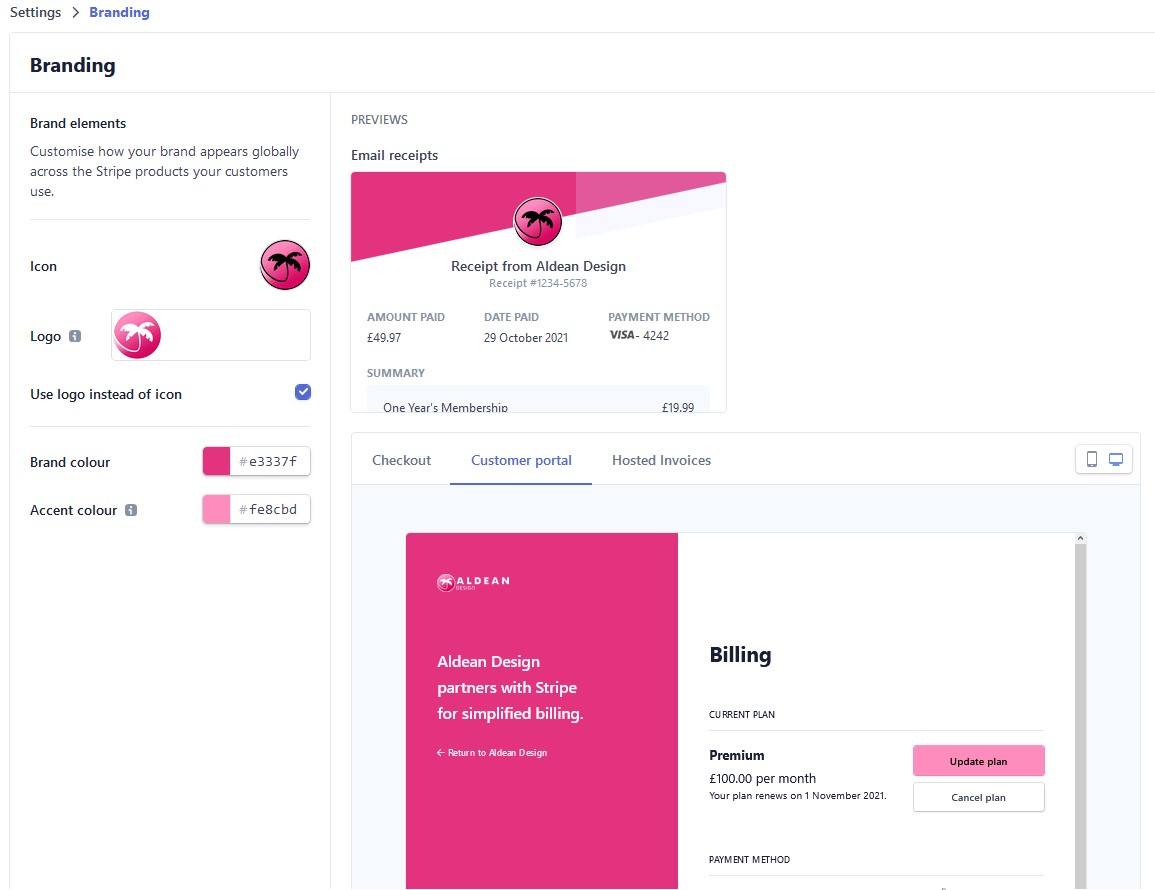
\includegraphics[width=1\linewidth]{graphics/stripe-customization.jpg}
	\caption{Customizing Stripe products using personal branding.}
	\vspace*{-5mm}
	\label{fig:stripe-customization}
\end{figure}
\pagebreak
	\section{Existing vertical jump calculators}
There are few \textit{modern} jump calculators on the market right now. None are combined with existing fitness platforms -
our research shows all of them being standalone mobile or web applications (\labelcref{research:fitness-meter,research:whats-my-vert,research:my-jump}).
\par
There are multiple methods of measuring jump height, often this is important to athletes 
where success is caused/correlated with jump ability i.e. Sprinting \cite{jump-sprint-link}, American football, Basketball, Volleyball.
We also know vertical jump is an important test to assess the explosive strength of the leg
musculature of athletes \cite{aspects-of-strength,nsa-strength-in-athletes}.
We'll be using the time-in-air (TIA) to estimate jump height. Whilst this is inevitably not perfectly
accurate, when using a force plate \footnote{A measuring instrument that measures the ground reaction forces generated by somebody.}
it is no worse than other methods (in terms of consistency) \cite{measuring-jump-paper}.
Thereby still proving useful to the target demographic.
\par
To summarise, the vertical jump calculator created for the project is intended for use as a measurement of progress
and not a concrete result. There will be some deviation from other measurements (such as using a \href{https://www.topendsports.com/testing/products/vertical-jump/vertec.htm}{Vertec}).
\pagebreak 

\subsection{Maths behind calculating vertical jump using video}
\label{research:jump-maths}
Below we'll be considering the physics \cite{hoopsgeek-maths} involved in finding vertical jump height using
\textbf{only smartphone video footage}.
\par
To explain the forces demonstrated in a countermovement jump (CMJ)\footnote{A vertical jump test performed by having an athlete quickly squat to a self-selected depth and then jump as high as possible.}
we'll be considering the 5 phases of action involved (\cref{fig:jump-phases}).
\begin{figure}[H]
	\centering
	\begin{minipage}[c]{0.5\textwidth}
		\caption{Motion phase of countermovement jump (CMJ). 1: Rest. Before jump. \linebreak2: Countermovement. 3: Push to ground. \linebreak4: Jump. Fly. 1 * : Rest. Land. \linebreak Vertical position of torso is y position \cite{jumping-phases-picture}.}
		\label{fig:jump-phases}
	\end{minipage}%
	\begin{minipage}[c]{0.5\textwidth}
		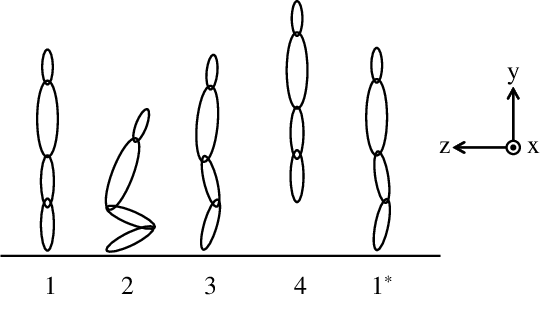
\includegraphics[width=\textwidth]{jump-maths/phases-of-cmj.png}
	\end{minipage}
\end{figure}
\vspace*{-5mm}
\begin{figure}[H]
	\centering
	\resizebox{0.7\linewidth}{!}{
    \noindent
    \begin{tikzpicture}[trim left=0cm]
        \centering
        \begin{axis}[
                axis on top,
                axis lines = left,
                xlabel = {time in seconds (s)},
                ylabel = {Force in Newtons},
                xmin=-1, xmax=1,
                ymin=0, ymax=2600,
                xtick={-1.0,-0.5,0.0,0.5,1.0},
                ytick={500,1000,1500,2000},
                axis line style={opaque},
                label style={font=\tiny},
                ticklabel style={font=\tiny},
                tick style={draw=none},
                legend style={draw=none},
            ]

            % Define axis lines
            % Gravity line defined
            \path [
                name path=axis,
            ]
            (axis cs:-1,0) -- (axis cs:1,0);


            % Gravity line defined
            \addplot [
                name path=gravity,
                color=gray,
                fill=gray!10!,
                draw=none,
                area legend,
            ]
            {1000};

            %Below the main force of jumper is defined
            \addplot [
                name path=A,
                domain=-1:1,
                samples=11,
                color=red,
                smooth,
                line width=1pt,
                tension={0.15}
            ]
            coordinates {
                    (-1,1000)(-0.6,1000)(-0.5,500)(-0.4,1000)(-0.3,1500)(-0.2,2000)(0.0,0.0)(0.5,0.0)(0.6,2100)(0.7,1250)(0.8,1600)(0.9,1000)(1,1000)
                };

            \addplot [
                name path=phase2end,
                domain=-0.6:-0.4,
                samples=11,
                opacity=0,
            ]
            coordinates {
                    (-0.4,1000)(-0.35,1250)(-0.205,2000)(0.0,0.0)(0.5,0.0)(0.6,2100)(0.7,1250)(0.8,1600)(0.9,1000)(1,1000)
                };

            \addplot [
                name path=phase3start,
                domain=-0.4:-0.2,
                samples=11,
                opacity=0,
            ]
            coordinates {
                    (-0.25,1000)(-0.25,1750)(-0.205,2000)(0.0,0.0)(0.5,0.0)(0.6,2100)(0.7,1250)(0.8,1600)(0.9,1000)(1,1000)
                };

            \addplot [
                name path=phase4start,
                domain=-0.4:-0.2,
                samples=11,
                opacity=0,
            ]
            coordinates {
                    (-0.1,1000)(0.0,0.0)(0.5,0.0)(0.6,2100)(0.7,1250)(0.8,1600)(0.9,1000)(1,1000)
                };


            \addplot [
                domain=0:0.5,
                samples=11,
                color=red,
                line width=2pt,
            ]
            coordinates {
                    (0,0)(0.5,0)
                };

            % Coloring the phase 1 decline blue
            \addplot [
                fill=blue,
                fill opacity = 0.2,
            ]
            fill between[
                    of=A and phase2end
                ];
            % Coloring the phase 1 incline orange
            \addplot [
                fill=orange,
                fill opacity = 0.2,
            ]
            fill between[
                    of=phase2end and phase3start
                ];
            % Coloring the phase 3 decline orange
            \addplot [
                fill=yellow,
                fill opacity = 0.2,
            ]
            fill between[
                    of=phase3start and phase4start
                ];
            % Coloring final phase
            \addplot [fill=green,fill opacity = 0.2] fill between[
                    of=A and gravity, soft clip={domain=0.55:1}
                ];

            % Coloring the gravity line
            \addplot [gray!10!] fill between[
                    of=A and axis, soft clip={domain=-1:-0.4}
                ];
            \addplot [gray!10!] fill between[
                    of=gravity and axis, soft clip={domain=-0.4:-0.1}
                ];
            \addplot [gray!10!] fill between[
                    of=A and axis, soft clip={domain=-0.1:0.55}
                ];
            \addplot [gray!10!] fill between[
                    of=gravity and axis, soft clip={domain=0.55:1}
                ];

            \legend{
                \tiny Force of Gravity,
                \tiny Force of Jumper Movement,
            }


            % The phase 1 bending label (70Ns)
            \addplot[mark=none, color = blue] coordinates {(-0.475,930)} node[pin=100:{\tiny 70Ns}]{} ;
            % Phase grey marks
            \addplot[mark=*, color=black!80!, draw opacity = 0] coordinates {(-0.6,1000)(-0.4,1000)(-0.26,1750)(0,0)(0.5,0)};
            % The phase 2 label (70Ns)
            \addplot[mark=none, color = orange] coordinates {(-0.31,1250)} node[pin=100:{\tiny 70Ns}]{} ;
            % The phase 3 label (245Ns)
            \addplot[mark=none, color = yellow] coordinates {(-0.16,1250)} node[pin=80:{\tiny 245Ns}]{} ;
            % The phase 4 label (245Ns)
            \addplot[mark=none, color = green] coordinates {(0.600,1250)} node[pin=100:{\tiny 245Ns}]{} ;


        \end{axis}
    \end{tikzpicture}}
	\vspace*{-5mm}
	\caption{Ground reaction forces during vertical jump.}
	\label{fig:jump-phases-graph}
\end{figure}
\pagebreak

We'll be using the above, simplified force plate analysis (\cref{fig:jump-phases-graph}),
to delve further into the phases of a jump and the mathematics. 
In reality the force curve wouldn't be so smooth
but this should demonstrate the phases quite clearly.
\par
\textbf{Phase 1: Rest (Pre-jump)}
\par
Before jumping we can see a flat line at $981$ Newton (\cref{fig:jump-phases-graph}). The athlete isn't jumping, but this is gravity doing it's
work. It's easily explained as $F=m*g$, where $m$ is the mass of the athlete and
$g$ is the acceleration of earth's gravity. $F$ is the force needed to counter the effects of gravity. We know that $g=9.81m/s^2$ on earth, thus:
\[
	\displaystyle
	\begin{aligned}
	981N &= m * 9.81 m/s^2 \\
	=> m &= \frac{981N}{9.81 m/s^2} = 100kg
	\end{aligned}	
\]
Here you can see that the force plate is basically acting as a weighing scale, showing
the force gravity exerts on the athlete.
\par
\textbf{Phase 2: Countermovement}
\par
As seen in \cref{fig:jump-phases}, the countermovement involves
the bending of the knees and typically swinging of the arms to lower the center
of gravity before the jump. The force plate (\cref{fig:jump-phases-graph}) is 
registering forces lower than 981N, which means the athlete is accelerating
in a downward movement.
\par
Recall Newton's 3rd Law of motion; 
which states whenever two objects interact, they exert equal and opposite forces on each other.
Knowing the above, we can define Ground Reaction Force (GRF) as ``the force exerted by the ground
on a body in contact with it''. 
We can describe the forces acting at this time as follows:
$$F_{Jumper} = F_{GRF} - F_{Gravity} <=0$$
We can also use the analysis (\cref{fig:jump-phases-graph}) to find
the speed the athlete is moving at before the jump. We know that
$F=ma$ (mass * acceleration), and force is happening over time.
Thus, $Ft=mat$.  
We also know force isn't a constant, it's a function of time and that we can define velocity as $v=at$;
so our formula is:
$$\displaystyle
\int_{t_1}^{t_2} F_{Jumper}(t) \mathrm{d}t = mv$$
where $F_{Jumper}(t)$ is the difference between the GRF and gravity.
\pagebreak
The integral can be calculated from the force plate data. The downward impulse\footnote{Impulse is the integral of a force.} made by
the athlete is shown in the graph (\cref{fig:jump-phases-graph}) as the blue area
below the line representing gravity.
\par
We've assumed the integral (impulse) is -70Ns\footnote{Newton seconds are the units of impulse.}. 
With this, we can conclude that:
\begin{align*}
& \int_{t_1}^{t_2} F(t) \mathrm{d}t = m v \\
&=> -70 N s = 100kg * v \\
&=> v = -70 N s / 100kg = -0.7 m/s
\end{align*}
Therefore, our athlete reaches a peak velocity of -0.7m/s during the countermovement phase.
\par
\textbf{Phase 2.5: Deceleration}
\par
Now we've seen where GRFs are lower than expected due to gravity - we must look for the period
where our athlete has to decelerate the downward movement (pause) before launching up (\cref{fig:jump-phases}).
This should be an equally big impulse to that found above but in the opposite direction.
We can describe this as:
\[\displaystyle \int_{t_2}^{t_3} F_{Jumper}(t) \mathrm{d}t = 70 Ns\]
Because we know $F(t)$ and $t_2$, the algorithm of the force plate analysis
now looks for $t_3$ so the impulse equals 70Ns.
\par
On our graph (\cref{fig:jump-phases-graph}) we have pictured this -
we are looking for the blue and orange areas to be the same size.
\par
\textbf{Phase 3: Push to ground}
\par
The athlete then generates force in preparation for takeoff before the GRFs register as 0
(when they are in flight). They reach some of the peak forces seen.
To assess the velocity during takeoff we use the same technique as Phase 2:
\[
\displaystyle
\int_{t_3}^{t_4} F_{Jumper}(t) \mathrm{d}t = mv	
\]
Pictured in our graph (\cref{fig:jump-phases-graph}) as the yellow area.
\pagebreak

The force plate graph detects 245Ns, so we can determine initial velocity as follows:
\vspace{-3mm}
\begin{align*}
	& 245 N s = 100kg * v \\
	&=> v = 245 N s / 100kg = 2.45 m/s
\end{align*}
\vspace{-5mm}

\textbf{Phase 4: Jump. Flight!}
Here the athlete can't control their velocity any longer; their jump height
is determined by the speed built before and during takeoff. Only gravity is acting on them,
bringing them back to the ground.
\par
We've determined initial velocity was $v(0)=2.45 m/s^2$ and
the gravity of earth has an acceleration of $a=9.81m/s^2$. Plus, the peak
of the jump must have a vertical velocity of zero: $v(t_{peak})=0$.
\par
Using the initial velocity and earths gravity we can find velocity at any given time using:
\vspace{-5mm}
\begin{center}
$
\displaystyle
v(t)=v(0) -a * t
$
\end{center}
\vspace{-5mm}
Thus we can find the velocity at the peak of the jump using:
\[\displaystyle
\begin{aligned}
v(t_{peak}) &= v(0) - a * t_{peak} \\
=> 0 &= v(0) - a * t_{peak} \\
=> t_{peak} &= \frac{v(0)}{a} = \frac{2.45m/s}{9.81m/s^2} = 0.25s
\end{aligned}\]
With the knowledge of $v(t)$ during every moment and knowing the peak of the jump
was 0.25s, we can calculate the jump height as the integral of velocity over the time
it takes to reach the peak of the jump:
\[\displaystyle
\begin{aligned}
h_{jump} &= \int_0^{\frac{v(o)}{a}} \bigg( v(o) - at \bigg) \ \mathrm{d}t= \\
& = v(o)t \ - \ \frac{1}{2} at^2 \ \bigg|_0^{\frac{v(0)}{a}} \\
& = v(0) \left(\frac{v(0)}{a}\right) - \frac{1}{2} a \left(\frac{v(0)}{a}\right)^2 \\
& = \frac{v(0)^2}{a} \ - \ \frac{1}{2} \frac{v(0)^2}{a} \\
=> h_{jump} \ &= \ \frac{1}{2} \frac{v(0)^2}{a} 
\end{aligned}\]
This leaves us with a simple formula for finding jump height
\textit{when we know the initial velocity}. 
For our force plate analysis (\cref{fig:jump-phases-graph}) we get
\[
	\begin{aligned}
		h_{jump} = \frac{1}{2} \frac{(2.45m/s)^2}{9.81 m/s^2} = 0.306m			
	\end{aligned}
\]

Because we only need the initial velocity of an athlete to satisfy our formula,
we don't have to rely on a force plate and expensive equipment.
We simply have to find the initial velocity for a jump that takes 0.5s.
\par
If someone jumps 0.5m high, they must also fall 0.5m after they peak. We have established
velocity is a linear function ($v=at$), thus we can demonstrate the athletes peak
is at the exact middle of the jump. Formally:
\vspace{-3mm}
\[
	\displaystyle
	t_{peak} = 0.5 * t_{hangtime}	
\]
Thus to find the jump height of someone who jumps for 0.5s, we can calculate
the distance of free fall in 0.25s!
\[
	\displaystyle
	\begin{aligned}
	S &= \int_0^{\frac{1}{2} t_{hangtime}} v(t) \; dt \\
	&= \int_0^{\frac{1}{2} t_{hangtime}} a * t \; dt \\
	&= \frac{1}{2} a t^2 \; \bigg|_0^{\frac{1}{2}t_{hangtime}} \\
	&= \frac{1}{2} a \left( \frac{1}{2} t_{hangtime} \right)^2 \\
	&= \frac{1}{8} a \: t_{hangtime}^2 \\
	\end{aligned}	
\]
In the case of a 0.5s hangtime, this gives us (as before with the force plate data):
\[
\begin{aligned}
	S = \frac{1}{8} a \: t_{hangtime}^2 = \frac{1}{8} * 9.81m/s^2 * 0.5^2 = 0.306m
\end{aligned}	
\]
\textbf{\underline{This formula is the crucial component to developing this feature.}} 
We won't be looking
at the physics of ``the landing'' in this document as it is not directly relevant.
However it is worth noting that to counteract the forces created during impact,
the athlete braces themselves and absorbs force - this is notable as the green area
in the graph has a value of 245Ns exactly like the yellow area.
\pagebreak

\subsection{FitnessMeter - Test \& Measure}
\label{research:fitness-meter}
\subsection{What's My Vertical?}
\label{research:whats-my-vert}
\subsection{My Jump 2}
\label{research:my-jump}


\begin{itemize}
	\item \href{https://www.thehoopsgeek.com/measurement-app/#manual}{HoopsGeek App}
	\item \href{https://apps.apple.com/us/app/fitnessmeter-test-measure/id477488986}{Old ass iphone app}
	\item \href{https://apps.apple.com/gb/app/my-jump-2/id1148617550#?platform=iphone}{MyJump2 itunes}
	\item \href{https://www.youtube.com/watch?v=tIBiHDyev6w}{MyJump2 in use}
	\item \href{https://www.topendsports.com/testing/products/vertical-jump/video.htm}{Maths}
	\item \href{https://www.thehoopsgeek.com/the-physics-of-the-vertical-jump/}{Detailed maths courtesy of thehoopsgeek - legend}
\end{itemize}
	\chapter{Project Specification}
\label{chap:project-specification}
\vspace{-10mm}
\section{Feature specification}
\label{sec:features}
The following is a summary of the core features we aim to provide; these will help in 
fulfilling the aims we set in \cref{chap:intro}.
\begin{itemize}[noitemsep]
    \item CRUD (Create, Read, Update, Delete) operations for a user account.
    \item A vertical jump calculator, operating via video upload (\textit{not recording through the app}).
    \begin{itemize}[nolistsep,noitemsep]
        \item Core: Scrub through the video to set the takeoff/landing point.
        \item Extra: Record video on the app (using the phone's camera).
    \end{itemize}
    \item Create a workout.
    \begin{itemize}[nolistsep,noitemsep]
        \item Core: From existing exercises.
        \item Extra: From custom uploaded exercises.
    \end{itemize} 
    \item Subscribe to a preset workout.
    \item A calendar for monitoring progress.
    \item A ``traffic light system'' for monitoring consistency.
    \item A means of communication with other users.
    \begin{itemize}[nolistsep,noitemsep]
        \item Potentially direct messaging or forum style messaging.
    \end{itemize}
    \item Provide video playback of exercises
    \item Allow measurement via metric \& imperial units (primarily for US users).
    \item Provide timer \& stopwatch functionality.
    \item Provide push notification reminders for calendar scheduled workouts.
    \item Provide notes functions for each workout.
    \begin{itemize}[nolistsep,noitemsep]
        \item Extra: Notes per exercise (allowing specific notes).
    \end{itemize}
\end{itemize}
\pagebreak


\section{Requirements}
\label{sec:requirements}
Using the above feature set (\cref{sec:features}), we can place features into functional requirements.
Other additional requirements will make up our non-functional requirements.
\vspace{-3mm}
\subsection{Functional requirements}
\begin{itemize}[noitemsep]
    \item CRUD for a User account.
    \item Upload video from storage.
    \item Scrub through video and set takeoff/landing.
    \item Calculate vertical jump in given units (metric or imperial).
    \item Support video(s) at different frame rate(s).
    \item Track vertical jump progress.
    \item Add/remove a workout to or from a user's calendar.
    \item Mark workouts as complete (with some visual feedback).
    \item Make notes regarding a specific workout.
    \item Provide push notification reminders at set duration(s) before a
    workout.
    \item Video playback from a source (embedded or from our own data storage).
    \item Stopwatch \& timer must work correctly.
    \item Simple chat/forum with other users.
    \item Calendar available on dashboard.
    \item Create a workout from existing exercises.
\end{itemize}
\subsection{Non-functional requirements}
\begin{itemize}[noitemsep]
    \item The app should be cross-platform (run on both iOS and Android).
    \item Have a consistent margin of error (under fixed conditions), when measuring vertical jump.
    \item Visualise workout consistency on user's dashboard.
    \item Operate smoothly and provide a close-to-native experience. Users must not
    feel delayed by the app if/when interviewed following usage.
    \item Aid users workout experience (aside from the vertical jump calculator).
    \item Be reliable (no unexpected data loss).
\end{itemize}
\pagebreak

\section{Technology Stack \& Considerations}
\subsection{Frontend technologies}
Given that the app will be cross-platform there are
a few largely accepted technologies for achieving this with a single codebase.
Namely, WebView frameworks (such as Apache Cordova, Ionic, and PhoneGap),
``React Native'' (created by Facebook) and ``Flutter'' (created by Google). 
\par
We'll be using \textbf{Flutter for the frontend} development for multiple reasons.
Commonly, developers opt to use React Native due to its large
community support - however in 2021, Flutter has a very similar ecosystem in my opinion.
Furthermore, whilst React Native is not noticeably slower than Flutter (in many cases) there is a fundamental
difference in how these software frameworks operate (and product native platform code from your high-level codebase).
React Native uses a JavaScript bridge to communicate between native code modules; on the other hand,
Flutter has native component availability by default - in practice the difference in performance is under
a second (milliseconds) but it's a consideration that holds weight as complexity of a project grows.
\par
Flutter is written using Dart (a rarely used language that is predominantly only used for Flutter development).
This is a stark change from JavaScript (used for React Native and more) which I have had previous experience with.
\textit{The project} is an opportunity for me to expand my skill set and learn to work with Dart when using
the Flutter framework - something which I have little experience with at present. Additionally,
JavaScript will be used for \textit{the product} during deployment.
\par
The final reason worth mentioning is Flutter comes with out-of-the-box testing features
as a framework - meaning there is less trouble finding a good workflow.
All of this in addition to the plethora of default UI components and APIs\footnote{Application programming interface(s)} means
that Flutter will be perfect for any form of iterative approach 
to software development.
\pagebreak

\subsection{Backend technologies}
For the backend data storage, \textbf{we'll be using MongoDB}
- the most popular NoSQL database currently in use.
In large part, this is being used as an opportunity for me
to utilise NoSQL databases as part of a large project as well as
learning to design NoSQL databases from scratch. Ordinarily
developers are typically assigned to projects that have been set-up
by other engineers thus they aren't typically involved in the
architectural stages of system design - including the considerations made when creating database schema.
\par
Personal motivation aside, NoSQL databases are hugely beneficial in a variety of ways.
Firstly, we have the ability to handle large amounts of data at high speeds.
This is achieved using a ``scale-out architecture'' - this simply means that instead
of relying on more computing power (as is the case in traditional ``scale-up architecture'')
we can scale by adding nodes. Related to this is the removal of SQL; not only
are we now avoiding potentially complex and inefficient queries but by
remove the ``SQL magic'' developers can focus on elegant application solutions instead
of spending precious development hours optimizing SQL queries for the database schema that
is in use.
\par
From a data perspective, NoSQL means we can store all kinds of data
structures (formally ``models'') instead of the SQL default tables, rows, columns.
MongoDB supports all forms of raw, semi-structured and structured data; this can be as simple
as binary data, to creating ``documents'' that represent highly structured data such as ``User accounts''
with multiple references.
\par
Overall MongoDB is being used primarily due to it being the most popular NoSQL database and the inherent
community support that coincides with this will be greatly beneficial during development.
It's important to note that poor implementation of NoSQL databases
can mean operating at shockingly slow speeds. Due to the nature of the flexibility and scalability
involved with these databases they are also more susceptible to duplicate data - it is much more difficult
to remove this redundancy than traditional relational models where we can follow a normalization process.
Often traditional normalization makes use of joins, which are not easily executed using MongoDB
and can easily lead to inferior code.
\pagebreak

\textbf{To expose the backend data for the apps to consume 
we'll be using Express.js} - a backend web application
framework for \textbf{Node.js} used in building APIs. Routing is simple and a fully functional
basic API can be written in under 100 lines of code. This level of detail
is not essential at this stage but noting our use of Express will hopefully
help in rationalizing the more high-level decisions outlined above.
\par
Naturally, the technology stack used may include other middle layer
technologies, but it's more than likely we focus our efforts on
Flutter \& MongoDB before further decisions.
For example, we may introduce a cache layer using Redis to optimize
queries and make our product more efficient. This iterative behavior is natural in 
software engineering and so there's an abundance of changes that can occur in our stack which will ease
development. This doesn't mean radical changes to our simple Flutter-Express-Node stack
but hopefully explains why it's difficult to document any packages and frameworks
we intend to use without a thorough system design stage (often taking months).
\vspace{-5mm}
\subsection{Security and deployment considerations}
The application backend will be hosted on the cloud using
AWS (Amazon Web Services). This is easier to set up than
self-hosting on dedicated servers and avoids the configuration needed to create
a secure system. The costs are predictable based on the usage we see, and
we can easily scale without having to invest in additional server hardware.
AWS is more configurable than other major cloud providers
but provides greater support versus IAC\footnote{Infrastructure-as-code}
tools like Terraform.
\par
We also plan on using fastlane as the CD component of the CI/CD pipeline for deployment.
GitHub Actions can also be used during growth stages before moving to a traditional
CI/CD tool like Jenkins - which can also be integrated with many AWS services. 
\par
A note must be made that many of the above technology decisions are made with HR in mind.
To explain this we must think further into the future; avoiding IAC means we're less likely
to need to employ cloud infrastructure engineers (thus reducing costs) and using popular technologies means
we won't struggle to find talent if needed. These decisions 
are largely dependent on what happens with the product and whether the concept
is proven as commercially viable, but that doesn't dismiss the need to account for factors
such as employee churn as early as possible.

	\chapter{Preliminary Work}
\label{chap:preliminary-work}
\vspace{-10mm}
\section{Software architecture}
\label{sec:architecture}
\begin{figure}[H]
    \centering
    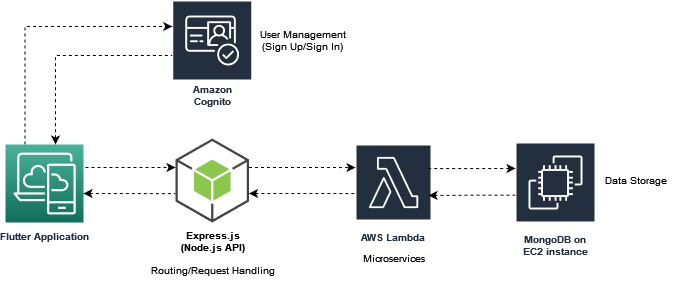
\includegraphics[width=\textwidth]{graphics/project-architecture.png}
    \caption{A high-level system architecture outlining basic interactions.}
    \label{fig:architecture-diagram}
\end{figure}
\vspace{-5mm}
Using an Express API inside AWS Lambda is beneficial because
AWS Lambda is an event-driven serverless platform. Instead of paying for cloud servers, you pay for compute power
that is proportional to the complexity of events taking place. For example,
we can process data on command instead of constantly having processes taking place.
This implementation can cause ``cold starts'' where there is some time wasted if the system hasn't been accessed
in a while, but the time spent is negligible for our project and the cost-benefit analysis would show
that this is a rationale decision. Using Amazon Cognito also removes much of the development
time needed to create simple user management. This doesn't require much skill and so making use of 
Amazon Cognito is saving us time to use where knowledge and focus is needed.
\pagebreak

\section{User interface design}
\label{sec:UI-design}
\vspace{-3mm}
We have created some preliminary designs (\cref{fig:prototype}) in the form of a functional prototype.
Main screens have been created and the overall aesthetic is displayed.
It's highly likely that the colour palette is changed to meet the brand
we decide to create for the application.\\
The functional prototype can be found here: \href{https://www.figma.com/proto/aANVZK2JZcBTPZCzaFYvbm/Final-Year-Project-Prototype?scaling=scale-down&page-id=0%3A1&starting-point-node-id=0%3A3&node-id=0%3A3}{Project Prototype Link}.
\vspace{-2mm}
\begin{figure}[H]
    \centering
    \begin{minipage}{0.5\textwidth}
        \begin{subfigure}{\textwidth}
            \centering
            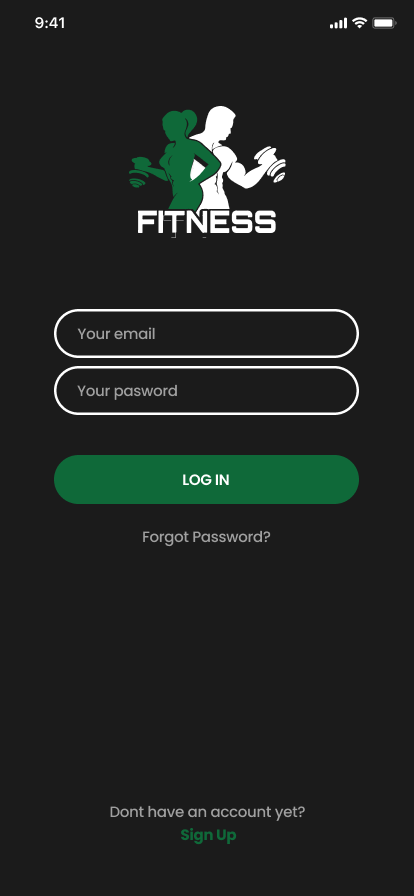
\includegraphics[width=0.45\textwidth]{graphics/prototype/login-page.png}
            \caption{Login screen}
            \label{fig:prototype-login}
        \end{subfigure}
    \end{minipage}%
    \begin{minipage}{0.5\textwidth}
        \begin{subfigure}{\textwidth}
            \centering
            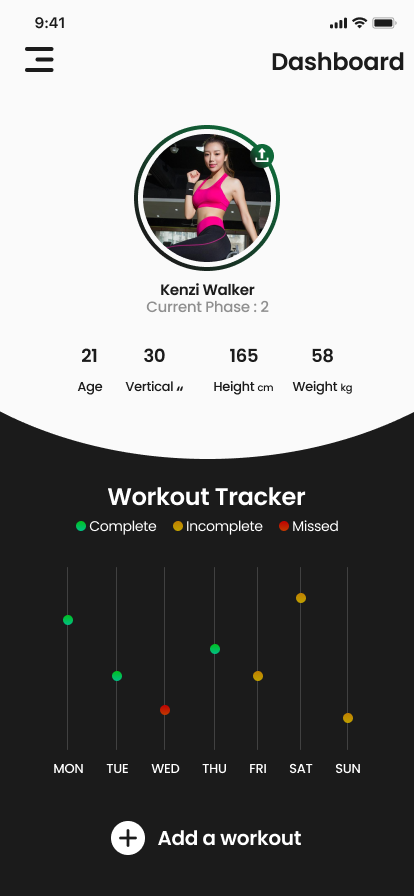
\includegraphics[width=0.45\textwidth]{graphics/prototype/dashboard.png}
            \caption{Main dashboard}
            \label{fig:prototype-dashboard}
        \end{subfigure}
    \end{minipage}\\*[3mm]
    \centering
    \begin{minipage}{0.5\textwidth}
        \begin{subfigure}{\textwidth}
            \centering
            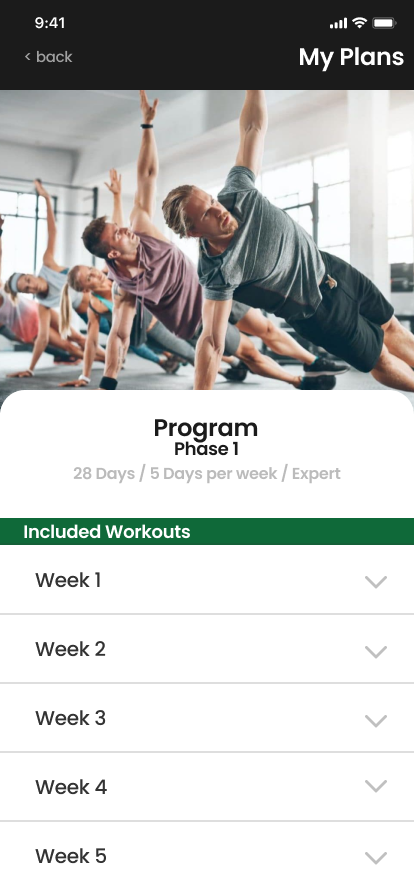
\includegraphics[width=0.45\textwidth]{graphics/prototype/workout-plan.png}
            \caption{Workout screen}
            \label{fig:prototype-workouts}
        \end{subfigure}
    \end{minipage}%
    \begin{minipage}{0.5\textwidth}
        \begin{subfigure}{\textwidth}
            \centering
            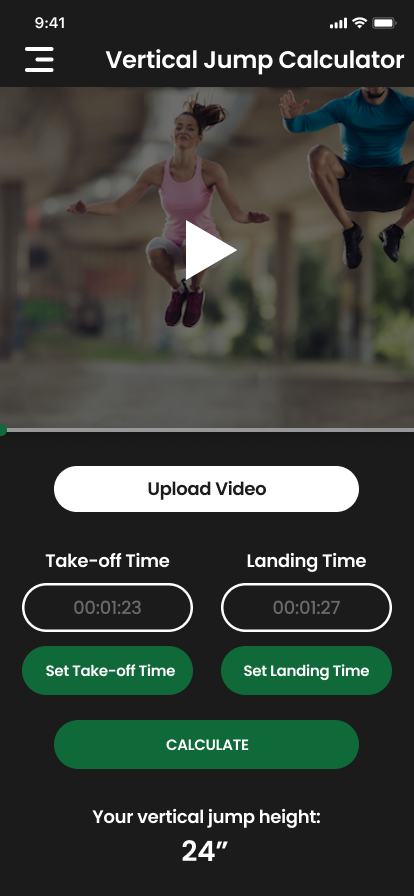
\includegraphics[width=0.45\textwidth]{graphics/prototype/jump-calc.png}
            \caption{Jump calculator screen}
            \label{fig:prototype-jump-calc}
        \end{subfigure}
    \end{minipage}%
    \caption{A selection of prototype screens.}
    \label{fig:prototype}
\end{figure}
	\chapter{Project Plan}
\label{chap:project-plan}

\section{Deliverables}
\label{sec:deliverables}
\vspace{-3mm}
\textbf{\underline{Final UI design \& brand guidelines}}
\par
\textbf{Due date:} 13/12/21
\par
\vspace{-3mm}
\textbf{Description:} The finalized branding and user interface designs for all major screens of the application.
These will be used during development for reference and to create reusable components (``widgets'' in Flutter) for consistency across
the application. The branding is also important for further marketing of \textit{the product} in future.
\par
\vspace{-3mm}
\textbf{Success criterion:} Easy-to-follow guidance for developers. No further questions
should be asked from developers as the guidance should be comprehensive enough for complete development.
\par

\textbf{\underline{Reusable UI Components (``Widgets'') - and test cases}}
\par
\textbf{Due date:} 24/12/21
\par
\vspace{-3mm}
\textbf{Description:} Custom Flutter widgets that complete the design system put forward in the guidelines. Any developer will use
these widgets to produce consistent frontend code. Custom test cases must be written to verify these function as normal (buttons etc.).
\par
\vspace{-3mm}
\textbf{Success criterion:} No errors should be found when using custom widgets in place of default widgets during early stage development. All Flutter widget tests should pass.
\par
\pagebreak

\textbf{\underline{Minimum Viable Product}}
\par
\textbf{Due date:} 31/01/22
\par
\vspace{-3mm}
\textbf{Description:} A fully functional and ready-to-test application that features all the core features. The bare minimum product
that could satisfy the aims we set in \cref{sec:intro_overview}. The overall
efficiency and elegance of the UI is not as crucial as the functionality at this stage.
\par
\vspace{-3mm}
\textbf{Success criterion:} Any stakeholder or external user could comfortably agree that the aims have been met when
using the app. It should be demonstrable.
\par

\textbf{\underline{Complete Test Suite(s)}}
\par
\textbf{Due date:} 14/02/22
\par
\vspace{-3mm}
\textbf{Description:} A comprehensive collection of tests for the Flutter application (and ideally for the Express API).
This should be composed of existing widget tests, unit tests for specific functionality and
integration tests for when the system is ready to be thoroughly tested. The ``system under test'' must be clearly defined where applicable.
\par
\vspace{-3mm}
\textbf{Success criterion:} Test coverage must cover all requirements set in \cref{sec:requirements} as well as architectural data paths
visualised in \cref{fig:architecture-diagram} (thorough structural coverage). Tests must satisfy that the features desired (\cref{sec:features}) are
tested and function as expected.
\par

\textbf{\underline{MVP Test Results}}
\par
\textbf{Due date:} 21/02/22
\par
\vspace{-3mm}
\textbf{Description:} Results and actions to take following the application of the test suite to the MVP.
\par
\vspace{-3mm}
\textbf{Success criterion:} All tests have actionable results - pass/fail must be accompanied by a relevant message describing
the outcome(s) and next steps (if any).
\par

\textbf{\underline{Project completion \& presentation created}}
\par
\textbf{Due date:} 15/03/22
\par
\vspace{-3mm}
\textbf{Description:} All relevant testing changes made. A presentation document should accompany the final product ready for demonstration
to stakeholders during the project fair. Usability and efficiency are not of utmost importance but should be prioritized.
\par
\vspace{-3mm}
\textbf{Success criterion:} A functional application that satisfies all aims and passes all test cases.
\par
\pagebreak

\textbf{\underline{Dissertation}}
\par
\textbf{Due date:} 03/05/22
\par
\vspace{-3mm}
\textbf{Description:} A documentation of the progress and development of the project through to completion. This forms a large portion of the basis
for grading of the project and the deadline is final.
\par
\vspace{-3mm}
\textbf{Success criterion:} A thoroughly well written document that describes the development process and lessons learnt from the project.

\vspace{-5mm}
\section{Project schedule}
\begin{figure}[H]
    \noindent\makebox[\textwidth]{
        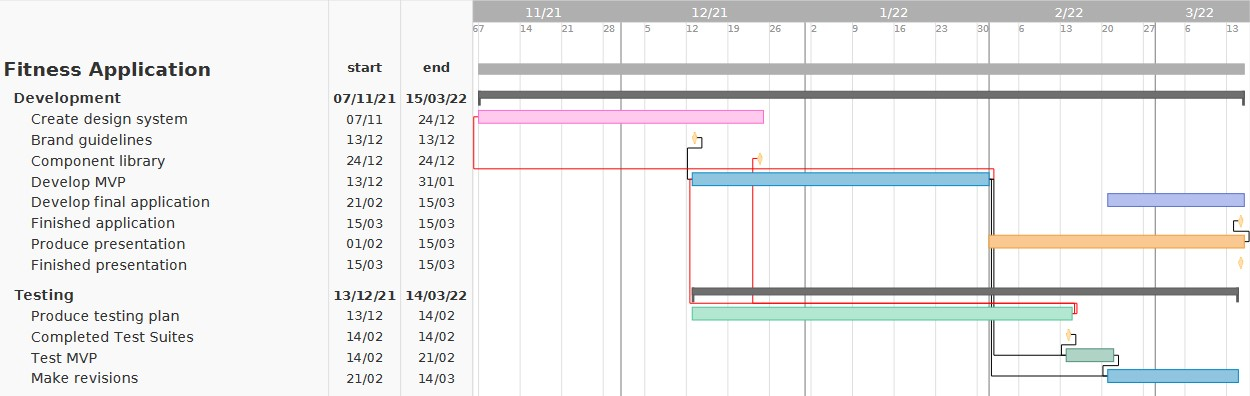
\includegraphics[width=1.2\textwidth]{graphics/gantt-chart.jpg}}
    \caption{An overview Gantt chart, clearly outlining milestones and phases.}
    \label{fig:gantt}
\end{figure}
\vspace{-5mm}
The project has begun already as seen in \cref{chap:preliminary-work}, however
we are using 07/11/21 as an acting ``start date''. We expect the project to be completed by
15/03/22. There is some float as seen in the above Gantt chart (\cref{fig:gantt});
mainly focused on the end of the MVP development phase and testing. Having some leverage
here means we can adjust our schedule dependent on the volume of changes that need to be implemented.
\vspace{-5mm}
\subsection{Limitations}
\vspace{-3mm}
Our main limitations are time and scope. As established in \cref{chap:intro},
the project is different and has a more narrow scope than \textit{the product}.
Spending too much time refining code and not focusing on implementation of complex features will mean
the grade achieved for the project is low(er) due to us not meeting the aims we have outlined in this document.
Time is a factor in this problem as it must be used wisely and we must aim to stick to the project schedule in order
to complete the core functionality (and by extension, the project) on time. These risks are assessed later (\cref{sec:risk}).
\pagebreak

\section{Software development strategy}
We intend on following a ``Feature-driven development'' (FDD) - an iterative and incremental software development
process. The rationale here is that the bulk of our success criterion rely on the features (functionality) of our
application. Focusing on establishing features first will mean we are more likely to
fulfill our aims - albeit at the expense of thorough testing during development.
\subsection{Choice of model}
As mentioned prior, FDD is an iterative process; it comfortably falls under the ``Agile'' methodology umbrella.
Agile models like FDD are more adaptable and mean that decisions can be made following short sprints of code without
drastic further impact on our project schedule and lifecycle. Whilst it's true that we run the risk of
making brash decisions, this can be mitigated by having regular reviews (stand-ups) and
in our case, sanity checks and meetings with the project supervisor(s) and other stakeholders.
\par
The decision to follow an Agile approach specifically is due to the tight deadlines and
unclear final product. By reviewing development frequently and focusing on developing features of the application we are
less likely to encounter scope creep and more likely to satisfy the success criteria we have established.
For the sake of argument, let's suppose we followed a traditional SDLC model (think Waterfall, Spiral, V-Shape).
We'd have to spend significant time outlining clear phases of our lifecycle and focusing on said phases in sequence (with most models).
This would mean less time is left for development before March and given the unfamiliarity with
the proposed technology stack this would dramatically increase the risk of not completing the application (or worse the MVP).
Adapting to roadblocks would also require pauses in development and alteration of our
predetermined phases (such as testing). This (again) increases our failure risk.
\par
Ultimately, whilst traditional SDLC models are sufficient for large-scale well-documented projects with
comprehensive feasibility reports and cost-benefit analyses - it is not ideal
when we are completing a project single-handedly under strong time constraints.
Deadlines are thoroughly fixed and without sacrificing performance
in the degree it would be difficult to follow said models well.
\pagebreak

\subsection{Testing lifecycle}
We'll be using aspects of ``Behaviour-driven Development'' (BDD) which is an extension of
``Test-driven Development''. Our use of BDD is only relevant to the testing approach we'll be following.
BDD testing uses human-readable descriptions of user requirements (similar to those in \cref{sec:requirements}) as the
basis for software tests. The process involves defining entities, events and outputs with given names before using
the names to encode system tests. Each test is based on a user story written using the aforementioned vocabulary.
For example:
\vspace{-5mm}
\begin{verbatim}
    Story: User can create a new exercise

    As an end user,
    In order to add new exercises
    I add video sources to a text description.

    On the create workout page,
    I press create new exercise,
    describe the exercise and add a video source
    before selecting "ok".
    Then my new exercise should appear
    as an option when creating a workout.
\end{verbatim}
\vspace{-5mm}
These tests are then translated into a programming language (in our case Dart code for Flutter)
to produce unit tests. We'll be following a black-box testing method, meaning
we aren't concerned with the internal workings behind the tests; we are only 
testing the functionality and not the implementation. This decouples
or tests from our code and means there is less to refactor if/when our code
is revised.
\par
For this project it's not likely we add much automation to our testing beyond where it is natural
such as widgets and other simple unit tests. Because deployment is outside of the scope of the project,
there is no significant reason to form a strong CI/CD pipeline.
\par
Our test results will be documented in a test summary report. This works similarly to this 
project proposal report and means that any stakeholder can read a brief report on how and what results were
found following our test phase. Following revisions, we will repeat the testing and add tests
if needed for future enhancements.

\section{Risk management plan}
\label{sec:risk}
We'll be using a risk register to document and describe risks below - this will form the single source where
risks can be documented and added/altered (based on changes in resources).
\par
\textbf{Risk description:} A description of the risk we're encountering.\\
\textbf{Probability of occurrence:} How likely the risk is to occur (using percentage).\\
\textbf{Severity:} The intensity of the risk on a 1-4 scale - low, medium, high, extremely high.\\
\textbf{Status:} View of the risk - potential, monitoring, occurring, or eliminated.\\
\textbf{Loss size (days):} Measuring the negative impact the occurrence of the risk would have.\\

\subsection{Risk analysis}
\textbf{Risk description:} File changes lost.\\
\vspace{-2mm}
\textbf{Probability of occurrence:} 5\%\\
\vspace{-2mm}
\textbf{Severity:} 1\\
\vspace{-2mm}
\textbf{Status:} potential\\
\vspace{-2mm}
\textbf{Loss size (days):} 1\\
\textbf{Mitigation strategy:} \cref{risk:mitigation-files}\\

\par

\hrulefill

\textbf{Risk description:} Behind on project schedule.\\
\vspace{-2mm}
\textbf{Probability of occurrence:} 50\%\\
\vspace{-2mm}
\textbf{Severity:} 2\\
\vspace{-2mm}
\textbf{Status:} monitoring\\
\vspace{-2mm}
\textbf{Loss size (days):} 7\\
\textbf{Mitigation strategy:} \cref{risk:mitigation-timeline}\\

\par

\hrulefill

\textbf{Risk description:} Scope creep.\\
\vspace{-2mm}
\textbf{Probability of occurrence:} 10\%\\
\vspace{-2mm}
\textbf{Severity:} 2\\
\vspace{-2mm}
\textbf{Status:} monitoring\\
\vspace{-2mm}
\textbf{Loss size (days):} 3\\
\textbf{Mitigation strategy:} \cref{risk:mitigation-scope}\\

\par

\pagebreak


\textbf{Risk description:} Contraction of COVID-19 or other illness.\\
\vspace{-2mm}
\textbf{Probability of occurrence:} 5\%\\
\vspace{-2mm}
\textbf{Severity:} 3\\
\vspace{-2mm}
\textbf{Status:} potential\\
\vspace{-2mm}
\textbf{Loss size (days):} 10\\
\vspace{-1mm}
\textbf{Mitigation strategy:} \cref{risk:mitigation-covid}\\


\hrulefill

\textbf{Risk description:} Travel delays without access to codebase.\\
\vspace{-2mm}
\textbf{Probability of occurrence:} 30\%\\
\vspace{-2mm}
\textbf{Severity:} 4\\
\vspace{-2mm}
\textbf{Status:} potential\\
\vspace{-2mm}
\textbf{Loss size (days):} 3\\
\textbf{Mitigation strategy:} \cref{risk:mitigation-travel}\\
\par

\hrulefill

\textbf{Risk description:} Technical knowledge roadblocks\\
\vspace{-2mm}
\textbf{Probability of occurrence:} 90\%\\
\vspace{-2mm}
\textbf{Severity:} 3\\
\vspace{-2mm}
\textbf{Status:} monitoring\\
\vspace{-2mm}
\textbf{Loss size (days):} 14\\
\textbf{Mitigation strategy:} \cref{risk:mitigation-roadblocks}\\
\par

\subsection{Risk mitigation}
\subsubsection{File changes lost:}
\label{risk:mitigation-files}
\vspace{-2mm}
This risk will be mitigated if encountered by using git version control and GitHub remote repositories.
The developer(s) will commit code periodically during development of features
and at minimum 1x per day (at COB \footnote{Close of business = 5pm}).

\subsubsection{Behind on project schedule:}
\label{risk:mitigation-timeline}
\vspace{-2mm}
The risk here is low given the float we have in our project schedule.
If this occurs then the bottleneck will be identified before considering
which other processes can continue simultaneously with finding a solution. This risk 
is prevalent during all stages of the project and avoidance is better than mitigation.
Mitigation strategies are largely dependent on identifying the bottleneck delaying the project.
In general this will involve trading off personal self-study for crisis resolution - the worst case is 1 complete week is lost
getting back on schedule.

\subsubsection{Scope creep:}
\label{risk:mitigation-scope}
\vspace{-2mm}
To avoid scope creep in the first instance, the project requirements will be tracked on a Kanban-style board during
feature-driven development. To mitigate any scope creep I will schedule regular sanity checks with my supervisor and
make use of ``rubber duck debugging'' to consciously hear what is being worked on.
Code reviews will take place via GitHub pull requests and the labelling of features
as ``enhancements'' will be used to mitigate the creeping in of new functionality and aims.

\subsubsection{Contraction of COVID-19 or other illness:}
\label{risk:mitigation-covid}
\vspace{-2mm}
I will actively avoid large gatherings and wear a mask where possible. I have received my 2nd vaccine and will
stay updated on the status of a booster vaccine if it provides sufficient efficacy
for avoiding covid-19. To mitigate the risk once contracted I will rest
and self isolate until recovered. This risk is one of the most difficult to mitigate as 
it involves personal health - without which I cannot actively work on the project.

\subsubsection{Travel delays without access to codebase:}
\label{risk:mitigation-travel}
\vspace{-2mm}
Being delayed during flights and trains without stable internet access is more than likely given
the global situation. To mitigate this risk I will use GitHub and carry a ``MiFi'' 4G router when travelling.
This means access to the code should be possible with just my GitHub credentials. In extreme circumstances,
I will clone the repository and work locally on a temporary machine before reaching home to comfortably push changes back.
I don't expect delays surpassing 3 days and there has been sufficient time allocated in the project schedule to 
limit the effects of any.

\subsubsection{Technical knowledge roadblocks:}
\label{risk:mitigation-roadblocks}
\vspace{-2mm}
This risk is inevitable given the project scope and development experience.
To mitigate this risk I will make extensive use of the Flutter forum(s) including
StackOverflow. This risk could mean the failure of the project - in which case
mitigation would involve drastically reframing the projects aims to be more achievable and avoid
the roadblock being encountered.


	\chapter{Summary}
We have looked at the project in adequate detail for stakeholders
to thoroughly understand the system being built. We've made a clear distinction between
future plans for \textit{the product} and the current plans for \textit{the project} (\cref{sec:intro_motivation}).
\par
To more broadly summarise, we'll be using Flutter and Express.js to 
implement the project described in \cref{chap:intro}. We'll
be using a Kanban-style project board with a feature-driven development model
to actively implement the features set out in \cref{sec:features}. The core focus
will be on the jump calculator as it's the unique aspect of the application being developed
and involves substantial difficulty when being created using frameworks for hybrid apps (as seen
by the lack of these frameworks and lack of cross-platform calculators) (\cref{chap:research}).
If time allows, we'll be implementing an ``administrator'' role for the application
as well as other extra features.
\par
This document has described at a high-level the entirety of the project plan,
however it's worth mentioning that a thorough cost-benefit analysis
and feasibility report as well as database and system design (in detail)
would add tremendous value to the development process. Whilst these are not 
explicitly required from this document, they would be near essential in a corporate environment
and would form the basis for the project proposal being accepted/rejected.
\par 
Given enough time (months, not weeks) to write a full project plan, we could collate a
fully comprehensive document detailing the technology choices, strategies and deployment methods
for developing a fitness application for training (with a vertical jump calculator).

	

% Insert the bibliography using citations contained in the file citations.bib
	\bibintoc % Whether to list the bibliography in the Table of Contents (or: \nobibintoc)
	\bibliography{citations} 
	
% In the appendix you might include a full code listing for an implemented algorithm 
% that you showed a small chunk of in one of your chapters. If you have extra graphs 
% you might enumerate them within the appendix and use \label{name} and \cref{name} 
% to automatically insert the correct section locations when you talk about them in your 
% chapters. It is *not* necessary to include all of your implementation code as an 
% appendix; instead, focus on the important highlights so they do not get drowned out.
% Within appendix.tex you should use chapters as the top level section dividers.
	% \ifdraftdoc\else
	% \appendix
	% \addappheadtotoc
	% % !TEX root = ../thesis.tex
\chapter{Implementation of a Relevant Algorithm}
\label{app:implementation_algorithm}

% Code listings should live in a code file, not embedded directly into your LaTeX code!
\lstinputlisting[language=c, caption={An implementation of an important algorithm from our work.}]{./listings/hello_world.c}


\chapter{Supplementary Data}
\label{app:supplementary_data}

The results of large ablative studies can often take up a lot of space, even with neat visualisation and formatting.
Consider putting full results in an appendix chapter and showing excerpts of interesting results in your chapters with detailed analysis.
You can use labels and references to refer the reader here for the full data.

	% \fi
	
\end{document}